\article{Eisenstein 级数与迹公式}{Eisenstein Series and the Trace Formula}{James Arthur}{1}{253--274}

\origsection{I}{Eisenstein 级数（Eisenstein series）}
Eisenstein 级数的谱理论（spectral theory）由 Selberg 开创，Langlands 在一份长期未刊、最近终于出版的手稿 [1] 中完成了这一理论。主要参考文献如下：
\begin{enumerate}
\item Langlands, \emph{On the functional equations satisfied by Eisenstein series}, Springer-Verlag, Berlin, 1976.
\item Langlands, \emph{Eisenstein series}, Algebraic Groups and Discontinuous Subgroups, Summer Research Institute (Univ. Colorado, 1965), Proc. Sympos. Pure Math., vol. 9, Amer. Math. Soc., Providence, R.I., 1966.
\item Harish-Chandra, \emph{Automorphic forms on semi-simple Lie groups}, Springer-Verlag, Berlin, 1968.
\end{enumerate}
本讲义的第一部分介绍这一理论的主要思想。

设 $G$ 是 $\Q$ 上的约化代数矩阵群（reductive algebraic matrix group）。那么 $G(A)$ 是各素位（valuation）$v$ 对应的群 $G(\Q_v)$ 的限制直积（restricted direct product）。若 $v$ 有限，且 $G(\mathfrak o_v)$ 是 $G(\Q_v)$ 的特殊极大紧子群（special maximal compact subgroup），则定义 $K_v=G(\mathfrak o_v)$。几乎所有素位都满足这一条件。对于其余有限 $v$，令 $K_v$ 为 $G(\Q_v)$ 的任一固定特殊极大紧子群。还固定一个定义在 $\Q$ 上的极小抛物子群（minimal parabolic subgroup）$P_0$，以及它的 Levi 分量（Levi component）$M_0$。令 $A_0$ 为 $M_0$ 中心中的极大分裂环面（maximal split torus）。令 $K_\R$ 为 $G(\R)$ 的一个固定极大紧子群，其 Lie 代数在 Killing 型下与 $A_0(\R)$ 的 Lie 代数正交。那么 $K=\prod_vK_v$ 为 $G(A)$ 的极大紧子群。

下文主要考虑标准抛物子群（standard parabolic subgroup），即定义在 $\Q$ 上且包含 $P_0$ 的抛物子群 $P$。固定这样的 $P$。令 $N_P$ 为 $P$ 的幺幂根基（unipotent radical），$M_P$ 为 $P$ 中包含 $M_0$ 的唯一 Levi 分量。于是 $M_P$ 中心的分裂分量（split component）$A_P$ 包含于 $A_0$。以 $X(M_P)_\Q$ 表示 $M_P$ 的 $\Q$ 有理特征群（character group），并定义
\[
 \mathfrak a_P=\operatorname{Hom}(X(M_P)_\Q,\R).
\]
若 $m=\prod_vm_v\in M(A)$，由
\[
 \exp\langle H_M(m),\chi\rangle=|\chi(m)|=\prod_v|\chi(m_v)|_v
\]
定义向量 $H_M(m)\in\mathfrak a_P$。令 $M_P(A)^1$ 为同态 $H_M$ 的核。那么 $M_P(A)$ 是 $M_P(A)^1$ 与 $A(\R)^0$ 的直积，后者为 $A(\R)$ 中单位元的连通分支。由于 $G(A)=N_P(A)M_P(A)K$，任意 $x\in G(A)$ 可写作 $nmk$，其中 $n\in N_P(A)$、$m\in M_P(A)$、$k\in K$。定义 $H_P(x)=H_M(m)\in\mathfrak a_P$。

令 $\Omega$ 为 $(G,A_0)$ 的限制 Weyl 群（restricted Weyl group）。它作用在 $\mathfrak a_0$ 的对偶空间上。在 $\mathfrak a_0$ 上固定一个正定且 $\Omega$ 不变的双线性型 $\langle\ ,\ \rangle$，从而将 $\mathfrak a_0$ 与其对偶等同。这使我们能把各 $\mathfrak a_P$ 嵌入 $\mathfrak a_0$。令 $\Sigma_P$ 为 $(P,A)$ 的根（root）的集合，即按 $A_P$ 的伴随作用（adjoint action）分解 $N_P$ 的 Lie 代数而得到的 $X(A)_\Q$ 中的元素。它们可看作 $\mathfrak a_P$ 中的向量。令 $\Phi_P$ 为 $(P,A)$ 的单根（simple root）集合。$G$ 本身也是抛物子群。分别把 $A_G$ 与 $\mathfrak a_G$ 记作 $Z$ 和 $\mathfrak z$。那么 $\Phi_P$ 是 $\mathfrak a_P$ 中 $\mathfrak z$ 的正交补的一组基。

设 $Q\subset P$ 是另一标准抛物子群。则 $Q^P=Q\cap M_P$ 为 $M_P$ 的抛物子群，其幺幂根基为 $N_Q^P=N_Q\cap M_P$。以 $\mathfrak a_Q^P$ 表示 $\mathfrak a_Q$ 中 $\mathfrak a_P$ 的正交补。一般地，与 $Q^P$ 相联系的对象以下标 $Q$、上标 $P$ 表示。例如，$\Phi_Q^P$ 是 $(Q^P,A_Q)$ 的单根集合，它是 $\Phi_{P_0}^P\backslash\Phi_{P_0}^Q$ 在 $\mathfrak a_Q^P$ 上的投影。以 $\widehat\Phi_Q^P$ 表示与 $\Phi_Q^P$ 对偶的 Euclid 空间 $\mathfrak a_Q^P$ 的基。若 $P_i$ 为抛物子群，常在上下标中以 $i$ 代替 $P_i$；若仅使用字母 $P$，也常省略其下标。最后，$\Q$ 上的群的 Lie 代数始终以小写哥特字母表示。

若 $P,P_1$ 是抛物子群，令 $\Omega(\mathfrak a,\mathfrak a_1)$ 为由 $\Omega$ 的元素限制到 $\mathfrak a$ 所得、从 $\mathfrak a$ 到 $\mathfrak a_1$ 的不同同构的集合。若此集合非空，则称 $P,P_1$ 相伴（associated）。设 $\mathcal P$ 是一个相伴类，且 $P\in\mathcal P$。称
\[
 \mathfrak a^+=\mathfrak a_P^+=\{H\in\mathfrak a:\langle\alpha,H\rangle>0,\ \alpha\in\Phi_P\}
\]
为 $P$ 在 $\mathfrak a$ 中的室（chamber）。

\begin{originaltheorem}{引理 1（Lemma 1）}
$\displaystyle\bigcup_{P_1\in\mathcal P}\bigcup_{s\in\Omega(\mathfrak a,\mathfrak a_1)}s^{-1}(\mathfrak a_1^+)$ 是一个不交并，且在 $\mathfrak a$ 中稠密。
\end{originaltheorem}

在讨论 Eisenstein 级数前，先定义一个诱导表示（induced representation）。固定 $P$。令 $\mathcal H_P^0$ 为函数
\[
 \Phi:N(A)\cdot M(\Q)\cdot A(\R)^0\backslash G(A)\longrightarrow\C
\]
所成的空间，满足：
\begin{enumerate}
\item[(i)] 对任意 $x\in G(A)$，函数 $m\mapsto\Phi(mx)$（$m\in M(A)$）是 $\mathfrak Z_{M(\R)}$ 有限的，其中 $\mathfrak Z_{M(\R)}$ 是 $\mathfrak m(\C)$ 的泛包络代数（universal enveloping algebra）的中心；
\item[(ii)] 由 $k\in K$ 索引的函数 $\Phi_k:x\mapsto\Phi(xk)$ 的张成空间有限维；
\item[(iii)] $\displaystyle\|\Phi\|^2=\int_K\int_{A(\R)^0M(\Q)\backslash M(A)}|\Phi(mk)|^2\,dm\,dk<\infty$。
\end{enumerate}
令 $\mathcal H_P$ 为 $\mathcal H_P^0$ 完备化得到的 Hilbert 空间。若 $\Lambda\in\mathfrak a_\C$（$\mathfrak a$ 的复化）、$\Phi\in\mathcal H_P$、$x,y\in G(A)$，置
\[
 (I_P(\Lambda,y)\Phi)(x)=\Phi(xy)
 \exp\langle\Lambda+\rho_P,H_P(xy)\rangle
 \exp(-\langle\Lambda+\rho_P,H_P(x)\rangle).
\]
这里 $\rho_P\in\mathfrak a$ 满足
\[
 |\det(\operatorname{Ad}m)_{\mathfrak n(A)}|
 =\exp\langle2\rho_P,H_M(m)\rangle,\qquad m\in M(A).
\]
$I_P(\Lambda)=I_P^G(\Lambda)$ 为 $G(A)$ 的一个表示，由 $P(A)$ 的一个表示诱导而来，后者又是 $M(A)$ 的某个表示（按我们的记号为 $I_M^M(\Lambda)$）的拉回。有
\[
 I_P(\Lambda,y)^*=I_P(-\bar\Lambda,y^{-1}),\qquad y\in G(A),
\]
以及
\[
 I_P(\Lambda,f)^*=I_P(-\bar\Lambda,f^*),\qquad f\in C_c^\infty(G(A)),
\]
其中 $f^*(y)=\overline{f(y^{-1})}$。特别地，$\Lambda$ 纯虚时，$I_P(\Lambda)$ 是酉表示（unitary representation）。

\paragraph*{注（Remark）.}
不难证明，$I_M^M(0)$ 是 $M(A)$ 在 $L^2(A(\R)^0\cdot M(\Q)\backslash M(A))$ 上的正则表示（regular representation）中离散分解的子表示。可写作
\[
 I_M^M(0)=\bigoplus_\iota\sigma^\iota,\qquad\sigma^\iota=\bigotimes_v\sigma_v^\iota,
\]
其中 $\sigma^\iota$ 为 $M(A)$ 的不可约表示。若 $v$ 为任意素数，$\sigma_v$ 为 $M(\Q_v)$ 的不可约酉表示，则定义
\[
 \sigma_{v,\Lambda}(m)=\sigma_v(m)\exp\langle\Lambda,H_M(m)\rangle,
 \qquad\Lambda\in\mathfrak a_\C,\ m\in M(\Q_v).
\]
把它提升到 $P(\Q_v)$ 再诱导到 $G(\Q_v)$，得到 $G(\Q_v)$ 的表示 $I_P(\sigma_v,\Lambda)$，作用于 Hilbert 空间 $\mathcal H_P(\sigma_v)$。由此记号，
\[
 I_P(\Lambda)=\bigoplus_\iota\bigotimes_vI_P(\sigma_v^\iota,\Lambda).
\]
因此，$I_P(\Lambda)$ 可完全用诱导表示与 $M$ 的离散谱理解。

固定 $P,P_1$，取 $s\in\Omega(\mathfrak a,\mathfrak a_1)$，令 $w_s$ 为 $s$ 在 $K\cap G(\Q)$ 与 $A_0$ 的正规化子之交中的固定代表。对 $\Phi\in\mathcal H_P^0$、$\Lambda\in\mathfrak a_\C$、$x\in G(A)$，考虑
\[
\begin{split}
 \int_{(N_1(A)\cap w_sN(A)w_s^{-1})\backslash N_1(A)}
 &\Phi(w_s^{-1}nx)\exp\langle\Lambda+\rho_P,H_P(w_s^{-1}nx)\rangle\,dn\\
 &\cdot\exp(-\langle s\Lambda+\rho_1,H_1(x)\rangle).
\end{split}
\]
约定：若 $H$ 是 $N_0$ 的任意闭连通子群，则 $dh$ 是使 $H(\Q)\backslash H(A)$ 体积为 $1$ 的 $H(A)$ 上的 Haar 测度。由此便唯一确定了上述商空间的测度 $dn$。

\begin{originaltheorem}{引理 2（Lemma 2）}
假设对每个 $\alpha\in\Sigma_P$，只要 $s\alpha\in-\Sigma_{P_1}$，就有
$\langle\alpha,\operatorname{Re}\Lambda-\rho_P\rangle>0$。那么上述积分绝对收敛。
\end{originaltheorem}
当 $\Lambda$ 满足引理条件时，这个积分定义一个从 $\mathcal H_P^0$ 到 $\mathcal H_{P_1}^0$ 的线性算子，记为 $M(s,\Lambda)$。交织积分（intertwining integral）在局部域上群的调和分析中起重要作用，所以 $M(s,\Lambda)$ 也自然地出现在整体理论中。

\begin{originaltheorem}{引理 3（Lemma 3）}
$M(s,\Lambda)^*=M(s^{-1},-s\bar\Lambda)$。此外，若
$f\in C_c^\infty(G(A))^K$，即 $C_c^\infty(G(A))$ 中 $K$ 共轭不变的函数，则\footnote{\textbf{译者注（本次校订）：}引理3的交织关系右端应为 $I_{P_1}(s\Lambda,f)M(s,\Lambda)$。由于 $M(s,\Lambda)$ 的目标空间是 $\mathcal H_{P_1}$，其后的表示须取在 $P_1$ 对应的空间上。}
\[
 M(s,\Lambda)I_P(\Lambda,f)=I_P(s\Lambda,f)M(s,\Lambda).
\]
\end{originaltheorem}
现在定义 Eisenstein 级数。
\begin{originaltheorem}{引理 4（Lemma 4）}
若 $\Phi\in\mathcal H_P^0$、$x\in G(A)$、$\Lambda\in\mathfrak a_\C$，且
$\operatorname{Re}\Lambda\in\rho_P+\mathfrak a^+$，则级数
\[
 E(x,\Phi,\Lambda)=\sum_{\delta\in P(\Q)\backslash G(\Q)}
 \Phi(\delta x)\exp\langle\Lambda+\rho_P,H_P(\delta x)\rangle
\]
绝对收敛。
\end{originaltheorem}

Eisenstein 级数的主要性质可概括为下面的定理。
\begin{originaltheorem}{主定理（Main theorem）}
(a) 设 $\Phi\in\mathcal H_P^0$。$E(x,\Phi,\Lambda)$ 与 $M(s,\Lambda)\Phi$ 可以作为亚纯函数（meromorphic function）解析延拓到 $\mathfrak a_\C$。在 $i\mathfrak a$ 上，$E(x,\Phi,\Lambda)$ 正则，$M(s,\Lambda)$ 酉。对 $f\in C_c^\infty(G(A))^K$ 和
$t\in\Omega(\mathfrak a_1,\mathfrak a_2)$，有函数方程：
\begin{enumerate}
\item[(i)] $\displaystyle E(x,I_P(\Lambda,f)\Phi,\Lambda)=\int_{G(A)}f(y)E(xy,\Phi,\Lambda)\,dy$；
\item[(ii)] $E(x,M(s,\Lambda)\Phi,s\Lambda)=E(x,\Phi,\Lambda)$；
\item[(iii)] $M(ts,\Lambda)\Phi=M(t,s\Lambda)M(s,\Lambda)\Phi$。
\end{enumerate}
(b) 令 $\mathcal P$ 为抛物子群的一个相伴类。以 $\widehat L_\mathcal P$ 表示可测函数
$F_P:i\mathfrak a\to\mathcal H_P$ 的族 $F=\{F_P:P\in\mathcal P\}$ 构成的集合，满足：
\begin{enumerate}
\item[(i)] 若 $s\in\Omega(\mathfrak a,\mathfrak a_1)$，则 $F_{P_1}(s\Lambda)=M(s,\Lambda)F_P(\Lambda)$；
\item[(ii)] $\displaystyle\|F\|^2=\sum_{P\in\mathcal P}n(A)^{-1}
 \left(\frac1{2\pi i}\right)^{\dim A}\int_{i\mathfrak a_P}\|F_P(\Lambda)\|^2\,d\Lambda<\infty$，
\end{enumerate}
其中 $n(A)$ 是 $\mathfrak a$ 中的室的个数。那么，把 $F$ 映为函数
\[
 \sum_{P\in\mathcal P}n(A)^{-1}\left(\frac1{2\pi i}\right)^{\dim A}
 \int_{i\mathfrak a}E(x,F_P(\Lambda),\Lambda)\,d\Lambda
\]
的映射，最初定义于 $\widehat L_\mathcal P$ 的一个稠密子空间，延拓为从 $\widehat L_\mathcal P$ 到
$L^2(G(\Q)\backslash G(A))$ 的一个闭 $G(A)$ 不变子空间
$L_\mathcal P^2(G(\Q)\backslash G(A))$ 的酉映射。此外，有正交分解
\[
 L^2(G(\Q)\backslash G(A))=\bigoplus_\mathcal P L_\mathcal P^2(G(\Q)\backslash G(A)).
\]
\end{originaltheorem}

这一定理表明，$G(A)$ 在 $L^2(G(\Q)\backslash G(A))$ 上的正则表示，是对抛物子群相伴类的一组代表 $\{P\}$ 求和的直和，每一项为直积分
$\int_{i\mathfrak a_P}^{\oplus}I_P(\Lambda)\,d\Lambda$。

定理的陈述简洁，证明却需要复杂的迂回论证。一种自然的思路是从任意 $\Phi\in\mathcal H_P^0$ 出发，直接证明 $M(s,\Lambda)\Phi$ 与 $E(x,\Phi,\Lambda)$ 的解析延拓；直接实行这一思路会遇到困难。对于一般 $\Phi$，直到 [1] 第231页，即 Langlands 原手稿的倒数第二页，才出现处理一般情形的方法。Langlands 的策略是，先对 $\mathcal H_P^0$ 的某个子空间 $\mathcal H_{P,\mathrm{cusp}}^0$ 中的 $\Phi$ 证明定理的所有相关陈述，再利用这一特殊情形逐步建立一般定理。

令 $\mathcal H_{P,\mathrm{cusp}}$ 为
$N(A)M(\Q)A(\R)^0\backslash G(A)$ 上的可测函数 $\Phi$ 的空间，满足
\begin{enumerate}
\item[(i)] $\displaystyle\|\Phi\|^2=\int_K\int_{M(\Q)A(\R)^0\backslash M(A)}|\Phi(mk)|^2\,dm\,dk<\infty$；
\item[(ii)] 对任意 $Q\subsetneq P$ 和 $x\in G(A)$，$\displaystyle\int_{N_Q(\Q)\backslash N_Q(A)}\Phi(nx)\,dn=0$。
\end{enumerate}
这是一个右 $G(A)$ 不变的 Hilbert 空间。
\begin{originaltheorem}{引理 5（Lemma 5）}
若 $f\in C_c^N(G(A))$，其中 $N$ 充分大，则映射 $\Phi\mapsto\Phi*f$（$\Phi\in\mathcal H_{G,\mathrm{cusp}}$）是 $\mathcal H_{G,\mathrm{cusp}}$ 上的 Hilbert--Schmidt 算子。
\end{originaltheorem}

将这个引理与紧算子的谱定理结合，便得到：
\begin{originaltheorem}{推论（Corollary）}
$\mathcal H_{G,\mathrm{cusp}}$ 分解为 $G(A)$ 的不可约表示的直和，每个表示的重数有限。
\end{originaltheorem}
$\mathcal H_{G,\mathrm{cusp}}$ 称为 $G(A)$ 上的尖点形式（cusp form）空间。把推论应用于 $M$，可知 $\mathcal H_{P,\mathrm{cusp}}$ 中任意函数都是 $\mathcal H_P^0$ 中函数的极限。因此，它是 $\mathcal H_P$ 的闭子空间，并在 $I_P(\Lambda)$ 下不变。

令 $\mathcal S(G)$ 为三元组 $\chi=(\mathcal P,\mathcal V,W)$ 的集合，其中 $W$ 为 $K$ 的不可约表示，$\mathcal P$ 为抛物子群相伴类，$\mathcal V$ 为子空间族
\[
 \{V_P\subset\mathcal H_{M,\mathrm{cusp}}^M\}_{P\in\mathcal P},
\]
这里 $\mathcal H_{M,\mathrm{cusp}}^M$ 为 $M(A)$ 上的尖点形式空间，且满足：
\begin{enumerate}
\item[(i)] 若 $P\in\mathcal P$，则 $V_P$ 是对应于 $\mathfrak Z_{M(\R)}$ 的某个复值同态的特征空间；
\item[(ii)] 若 $P,P_1\in\mathcal P$、$s\in\Omega(\mathfrak a,\mathfrak a_1)$，则 $V_{P_1}$ 是把 $V_P$ 中函数以 $w_s$ 共轭所得到的函数空间。
\end{enumerate}
若 $P\in\mathcal P$，定义 $\mathcal H_{P,\chi}$ 为 $\mathcal H_{P,\mathrm{cusp}}^0$ 中那些函数 $\Phi$ 的空间，使对每个 $x\in G(A)$：
\begin{enumerate}
\item[(i)] 函数 $k\mapsto\Phi(xk)$（$k\in K$）为 $W$ 的矩阵系数（matrix coefficient）；
\item[(ii)] 函数 $m\mapsto\Phi(mx)$（$m\in M(A)$）属于 $V_P$。
\end{enumerate}
$\mathcal H_{P,\chi}$ 是有限维空间，且对任意 $f\in C_c^\infty(G(A))^K$，在 $I_P(\Lambda,f)$ 下不变。$\mathcal H_{P,\mathrm{cusp}}$ 是所有满足 $P\in\mathcal P$ 的 $\chi=(\mathcal P,\mathcal V,W)$ 所对应的空间 $\mathcal H_{P,\chi}$ 的正交直和。

固定 $\chi=(\mathcal P,\mathcal V,W)$ 和 $P\in\mathcal P$。设有从 $\mathfrak a_\C$ 到有限维空间 $\mathcal H_{P,\chi}$ 的 Paley--Wiener 型解析函数
\[
 \Lambda\longmapsto\Phi(\Lambda)=\Phi(\Lambda,x),
 \quad\Lambda\in\mathfrak a_\C,\quad x\in N(A)M(\Q)A(\R)^0\backslash G(A).
\]
那么
\[
 \phi(x)=\left(\frac1{2\pi i}\right)^{\dim A}
 \int_{\operatorname{Re}\Lambda=\Lambda_0}
 e^{\langle\Lambda+\rho_P,H_P(x)\rangle}\Phi(\Lambda,x)\,d\Lambda
\]
是 $N(A)M(\Q)\backslash G(A)$ 上与点 $\Lambda_0\in\mathfrak a$ 无关的函数。沿 $x$ 的 $A(\R)^0$ 分量，它的支集是紧的。

\begin{originaltheorem}{引理 6（Lemma 6）}
对上述 $\Phi$，函数
\[
 \widehat\phi(x)=\sum_{\delta\in P(\Q)\backslash G(A)}\phi(\delta x)
\]
绝对收敛，并属于 $L^2(G(\Q)\backslash G(A))$。以 $L_\chi^2(G(\Q)\backslash G(A))$ 表示所有此类 $\widehat\phi$ 生成的闭子空间。那么有正交分解
\[
 L^2(G(\Q)\backslash G(A))=\bigoplus_{\chi\in\mathcal S(G)}L_\chi^2(G(\Q)\backslash G(A)).
\]
\end{originaltheorem}
\noindent\textit{译注：引理6的求和下标在原书印作 $P(\Q)\backslash G(A)$；紧接下文的同一求和使用 $P(\Q)\backslash G(\Q)$。此处保留原式。}

假设 $\Lambda_0\in\rho_P+\mathfrak a^+$。那么
\[
\begin{split}
 \widehat\phi(x)
 &=\left(\frac1{2\pi i}\right)^{\dim A}
 \int_{\operatorname{Re}\Lambda=\Lambda_0}
 \sum_{\delta\in P(\Q)\backslash G(\Q)}
 e^{\langle\Lambda+\rho_P,H_P(\delta x)\rangle}\Phi(\Lambda,\delta x)\,d\Lambda\\
 &=\left(\frac1{2\pi i}\right)^{\dim A}
 \int_{\operatorname{Re}\Lambda=\Lambda_0}E(x,\Phi(\Lambda),\Lambda)\,d\Lambda.
\end{split}
\]
设 $\Phi_1(\Lambda_1,x)$ 为与 $P_1$ 相联系的另一个函数。我们希望用 $\Phi,\Phi_1$ 表示内积
\[
 \int_{G(\Q)\backslash G(A)}\widehat\phi(x)\overline{\widehat\phi_1(x)}\,dx.
\]
该内积为
\[
\begin{split}
 &\int_{G(\Q)\backslash G(A)}\sum_{\delta\in P_1(\Q)\backslash G(\Q)}
 \widehat\phi(x)\overline{\phi_1(\delta x)}\,dx\\
 &=\int_{P_1(\Q)\backslash G(A)}\widehat\phi(x)\overline{\phi_1(x)}\,dx\\
 &=\left(\frac1{2\pi i}\right)^{\dim A_1}
 \int_{\operatorname{Re}\Lambda=\Lambda_0}\int_K
 \int_{A_1(\R)^0M_1(\Q)\backslash M_1(A)}\int_{A_1(\R)^0}
 E(namk,\Phi(\Lambda),\Lambda)\\
 &\hspace{30mm}\cdot e^{-2\langle\rho_1,H_1(x)\rangle}
 \overline{\phi_1(amk)}\,da\,dm\,dk.
\end{split}
\]

\begin{originaltheorem}{引理 7（Lemma 7）}
假设 $P,P_1$ 同秩。若 $\Phi\in\mathcal H_{P,\chi}$ 且
$\operatorname{Re}\Lambda\in\rho_P+\mathfrak a^+$，则
\[
 \int_{N_1(\Q)\backslash N_1(A)}E(nx,\Phi,\Lambda)\,dn
 =\sum_{s\in\Omega(\mathfrak a,\mathfrak a_1)}
 (M(s,\Lambda)\Phi)(x)e^{\langle s\Lambda+\rho_1,H_1(x)\rangle}.
\]
\end{originaltheorem}
若 $\Omega(\mathfrak a,\mathfrak a_1)$ 为空，即 $P,P_1$ 不相伴，则右端为零。
\begin{proof}
令 $\{\Omega\}$ 为满足对每个 $\alpha\in\Phi_0^P$ 均有 $s^{-1}\alpha>0$ 的 $s\in\Omega$ 的集合。那么它是 $\Omega$ 对 $M$ 的 Weyl 群的左陪集的一组代表。由 Bruhat 分解（Bruhat decomposition），
\[
\begin{split}
 &\int_{N_1(\Q)\backslash N_1(A)}E(nx,\Phi,\Lambda)\,dn\\
 &=\sum_{t\in\{\Omega\}}\int_{N_1(\Q)\backslash N_1(A)}
 \sum_{\nu\in(w_t^{-1}P(\Q)w_t\cap N_0(\Q))\backslash N_0(\Q)}
 \Phi(w_t\nu nx)e^{\langle\Lambda+\rho_P,H_P(w_t\nu nx)\rangle}\,dn.
\end{split}
\]
$w_tN_1w_t^{-1}\cap M$ 是 $M$ 的一个标准抛物子群的幺幂根基。若这个抛物子群不是 $M$ 本身，则由于 $\Phi$ 尖点，对应项为零。它为 $M$ 本身，当且仅当 $s=t^{-1}$ 将 $\mathfrak a$ 映到 $\mathfrak a_1$。此时
\[
 (w_t^{-1}Pw_t\cap N_0)\backslash N_0
 \simeq(w_t^{-1}Nw_t\cap N_1)\backslash N_1.
\]
因而上述公式等于
\[
\begin{split}
 \sum_{s\in\Omega(\mathfrak a,\mathfrak a_1)}
 &\operatorname{vol}\bigl((w_sN(\Q)w_s^{-1}\cap N(\Q))\backslash
 w_sN(A)w_s^{-1}\cap N(A)\bigr)\\
 &\cdot\int_{(w_sN(A)w_s^{-1}\cap N(A))\backslash N(A)}
 \Phi(w_s^{-1}nx)e^{\langle\Lambda+\rho_P,H_P(w_s^{-1}nx)\rangle}\,dn.
\end{split}
\]
按测度的选择，体积为 $1$，引理得证。\footnote{\textbf{译者注（本次校订）：}本证明最后一个式子中，与 $w_sNw_s^{-1}$ 相交的群，以及外层积分所用的群，都应为 $N_1$，以与引理中的 $N_1$ 常数项及交织算子的定义一致。引理前的内积展开还漏写了 $\int_{N_1(\Q)\backslash N_1(A)}\cdots\,dn$，其中的自由变量 $n$ 正应在这个商空间上积分。}
\end{proof}
结合引理与 Fourier 反演公式（Fourier inversion formula），有：
\begin{originaltheorem}{推论（Corollary）}
设 $P,P_1$ 相伴，$\phi,\phi_1$ 如引理7之前的讨论。则
\[
\begin{split}
 \int_{G(\Q)\backslash G(A)}\widehat\phi(x)\overline{\widehat\phi_1(x)}\,dx
 =\left(\frac1{2\pi i}\right)^{\dim A}
 \int_{\Lambda_0+i\mathfrak a}\sum_{s\in\Omega(\mathfrak a,\mathfrak a_1)}
 (M(s,\Lambda)\Phi(\Lambda),\Phi_1(-s\bar\Lambda))\,d\Lambda,
\end{split}
\]
其中 $\Lambda_0$ 可为 $\rho_P+\mathfrak a^+$ 中任意一点。
\end{originaltheorem}

引理1--6可由较为标准的估计证明。主定理的主要困难从这里开始，证明分为两个阶段。第一阶段是对 $\Phi\in\mathcal H_{P,\mathrm{cusp}}^0$ 完成解析延拓与函数方程。[2] 已很好地描述了这一部分，因此这里完全略过。第二阶段在 [1] 第7章完成，即 $L_\chi^2(G(\Q)\backslash G(A))$ 的谱分解；由此便推出主定理其余陈述。下面介绍这一论证的基本思路。

固定 $\chi=(\mathcal P_\chi,\mathcal V_\chi,W)$。[1] 第7章的论证建立在关于 $\dim(A/Z)$（$P\in\mathcal P_\chi$）的复杂归纳上。对 $\Phi\in\mathcal H_{P,\chi}$，假定 $E(x,\Phi,\Lambda)$ 和 $M(s,\Lambda)\Phi$ 在 $\mathfrak a_\C$ 上亚纯。证明过程中还说明，两者的奇点位于形如
\[
 \mathfrak r=\{\Lambda\in\mathfrak a_\C:\langle\alpha,\Lambda\rangle=\mu\},
 \qquad\mu\in\C,\ \alpha\in\Sigma_P
\]
的超平面上，并且仅有限多个这样的 $\mathfrak r$ 与
\[
 \mathfrak a^++i\mathfrak a
 =\{\Lambda\in\mathfrak a_\C:\langle\alpha,\operatorname{Re}\Lambda\rangle>0,
 \ \alpha\in\Phi_P\}
\]
相交。

令 $L_{\mathcal P_\chi,\chi}^2(G(\Q)\backslash G(A))$ 为由如下 $\widehat\phi(x)$ 生成的闭子空间：它们来自上述 $\Phi(\Lambda)$，且 $\Phi$ 在与 $\mathfrak a^++i\mathfrak a$ 相交的有限个奇异超平面上消失。若 $\phi_1(x)$ 来自 $\Phi_1(\Lambda_1)$，$P_1\in\mathcal P_\chi$，则可对内积公式应用 Cauchy 定理，得到
\[
 \left(\frac1{2\pi i}\right)^{\dim A}\int_{i\mathfrak a}
 \sum_{s\in\Omega(\mathfrak a,\mathfrak a_1)}
 (M(s,\Lambda)\Phi(\Lambda),\Phi_1(s\Lambda))\,d\Lambda,
\]
因为在 $i\mathfrak a$ 上有 $-s\bar\Lambda=s\Lambda$。在积分与求和中作变量代换，得到\footnote{\textbf{译者注（本次校订）：}下方变量代换的第一行，内积第二项应为 $\Phi_1(st\Lambda)$，而非 $\Phi_1(t\Lambda)$；下一行令 $r=st$ 后，才得到 $\Phi_1(r\Lambda)$。}
\[
\begin{aligned}
 &\left(\frac1{2\pi i}\right)^{\dim A}n(A)^{-1}
 \sum_{P_2\in\mathcal P_\chi}\sum_{t\in\Omega(\mathfrak a_2,\mathfrak a)}
 \sum_{s\in\Omega(\mathfrak a,\mathfrak a_1)}
 \int_{i\mathfrak a_2}(M(s,t\Lambda)\Phi(t\Lambda),\Phi_1(t\Lambda))\,d\Lambda\\
 &=\left(\frac1{2\pi i}\right)^{\dim A}n(A)^{-1}
 \sum_{P_2}\sum_{r\in\Omega(\mathfrak a_2,\mathfrak a_1)}
 \sum_{t\in\Omega(\mathfrak a_2,\mathfrak a)}
 \int_{i\mathfrak a_2}(M(rt^{-1},t\Lambda)\Phi(t\Lambda),\Phi_1(r\Lambda))\,d\Lambda\\
 &=\left(\frac1{2\pi i}\right)^{\dim A}n(A)^{-1}\sum_{P_2}\sum_r\sum_t
 \int_{i\mathfrak a_2}(M(t,\Lambda)^{-1}\Phi(t\Lambda),
 M(r,\Lambda)^{-1}\Phi_1(r\Lambda))\,d\Lambda\\
 &=\sum_{P_2\in\mathcal P_\chi}n(A)^{-1}
 \left(\frac1{2\pi i}\right)^{\dim A}\int_{i\mathfrak a_2}
 (F_{P_2}(\Lambda),F_{1,P_2}(\Lambda))\,d\Lambda,
\end{aligned}
\]

其中
\begin{equation}
 F_{1,P_2}(\Lambda)=\sum_{r\in\Omega(\mathfrak a_2,\mathfrak a_1)}
 M(r,\Lambda)^{-1}\Phi_1(r\Lambda),\tag{1}
\end{equation}
$F_{P_2}$ 类似定义。以 $\widehat L_{\mathcal P_\chi,\chi}$ 表示主定理中定义的 $\widehat L_{\mathcal P_\chi}$ 中、满足每个 $F_{P_2}$ 取值于 $\mathcal H_{P_2,\chi}$ 的函数族组成的子空间。上面的计算给出了从其一个稠密子空间到
$L_{\mathcal P_\chi,\chi}^2(G(\Q)\backslash G(A))$ 的一个稠密子空间的等距同构。

设 $\{F_{P_2}\}$ 为 $\widehat L_{\mathcal P_\chi,\chi}$ 中每个分量都光滑且紧支的函数族，$h(x)$ 为上述同构定义的对应函数。要证明 $h(x)$ 等于
\[
 h'(x)=\sum_{P_2\in\mathcal P_\chi}n(A_2)^{-1}
 \left(\frac1{2\pi i}\right)^{\dim A}
 \int_{i\mathfrak a_2}E(x,F_{P_2}(\Lambda),\Lambda)\,d\Lambda.
\]
对上述 $\widehat\phi_1(x)$，引理7推论的同一论证说明
\[
\begin{split}
 &\int_{G(\Q)\backslash G(A)}h'(x)\overline{\widehat\phi_1(x)}\,dx\\
 &\quad=\sum_{P_2}n(A_2)^{-1}\left(\frac1{2\pi i}\right)^{\dim A_2}
 \int_{i\mathfrak a_2}\sum_{r\in\Omega(\mathfrak a_2,\mathfrak a_1)}
 (M(r,\Lambda)F_{P_2}(\Lambda),\Phi_1(r\Lambda))\,d\Lambda.
\end{split}
\]
由于 $\widehat\phi_1$ 在 $L_{\mathcal P_\chi,\chi}^2$ 上的投影对应于 (1) 中的 $\{F_{1,P_2}\}$，该式等于
\[
\begin{split}
 &\sum_{P_2}n(A_2)^{-1}\left(\frac1{2\pi i}\right)^{\dim A_2}
 \int_{i\mathfrak a_2}(F_{P_2}(\Lambda),F_{1,P_2}(\Lambda))\,d\Lambda\\
 &=\int_{G(\Q)\backslash G(A)}h(x)\overline{\widehat\phi_1(x)}\,dx.
\end{split}
\]
于是证明了 $h=h'$，完成 Langlands 归纳的第一阶段。

在第二阶段，Langlands 令 $Q$ 为 $L_\chi^2(G(\Q)\backslash G(A))$ 到
$L_{\mathcal P_\chi,\chi}^2(G(\Q)\backslash G(A))$ 的正交补上的投影。对于对应于 $\Phi(\Lambda),\Phi_1(\Lambda_1)$ 的任意 $\widehat\phi,\widehat\phi_1$，内积 $(Q\widehat\phi,\widehat\phi_1)$ 等于
\[
\begin{split}
 \left(\frac1{2\pi i}\right)^{\dim A}\Bigg(&
 \int_{\Lambda_0+i\mathfrak a}\sum_{s\in\Omega(\mathfrak a,\mathfrak a_1)}
 (M(s,\Lambda)\Phi(\Lambda),\Phi_1(-s\bar\Lambda))\,d\Lambda\\
 &-\int_{i\mathfrak a}\sum_s
 (M(s,\Lambda)\Phi(\Lambda),\Phi_1(-s\bar\Lambda))\,d\Lambda\Bigg).
\end{split}
\]
选择 $\mathfrak a^+$ 中从 $\Lambda_0$ 到 $0$ 的一条路径，使它与
$\{M(s,\Lambda):s\in\Omega(\mathfrak a,\mathfrak a_1)\}$ 的每个奇异超平面 $\mathfrak r$ 至多交于一点 $Z(\mathfrak r)$。每个这样的 $\mathfrak r$ 具有形式
$X(\mathfrak r)+\mathfrak r_\C^\vee$，其中 $\mathfrak r^\vee$ 为实余维 $1$ 子空间，$X(\mathfrak r)\in\mathfrak a$ 与它正交。点 $Z(\mathfrak r)$ 属于
$X(\mathfrak r)+\mathfrak r^\vee$。由留数定理（residue theorem），内积等于
\[
 \left(\frac1{2\pi i}\right)^{\dim A-1}\sum_\mathfrak r
 \int_{Z(\mathfrak r)+i\mathfrak r^\vee}
 \sum_{s\in\Omega(\mathfrak a,\mathfrak a_1)}
 \operatorname{Res}_\mathfrak r(M(s,\Lambda)\Phi(\Lambda),\Phi_1(-s\bar\Lambda))\,d\Lambda.
\]
接下来重复第一阶段的步骤：把 $\Lambda_0$ 换为 $Z(\mathfrak r)$，$0$ 换为 $X(\mathfrak r)$，而 $E(x,\Phi,\Lambda)$ 换为 $\operatorname{Res}_\mathfrak r E(x,\Phi,\Lambda)$。

假设对某个单根 $\alpha\in\Phi_P$，有
$\mathfrak r^\vee=\{H\in\mathfrak a:\langle\alpha,H\rangle=0\}$。那么 $\mathfrak r^\vee=\mathfrak a_R$，其中 $R$ 是包含 $P$ 的抛物子群。对 $\Phi\in\mathcal H_{P,\chi}$，定义
\[
 E^R(x,\Phi,\Lambda)=\sum_{\delta\in P(\Q)\backslash R(\Q)}
 \Phi(\delta x)e^{\langle\Lambda+\rho_P,H(\delta x)\rangle}.
\]
它本质上是由 $M_R(A)$ 上的尖点数据构造的 Eisenstein 级数，对适当的 $\Lambda\in\mathfrak a_\C$ 收敛，且可亚纯延拓。显然，只要右端收敛，就有
\[
 E(x,\Phi,\Lambda)=\sum_{\delta\in R(\Q)\backslash G(\Q)}E^R(\delta x,\Phi,\Lambda).
\]
设 $\Lambda\in\mathfrak r$，且
$\Lambda=X(\mathfrak r)+\Lambda^\vee$，$\Lambda^\vee\in\mathfrak r_\C^\vee$，
$\operatorname{Re}\Lambda^\vee\in\rho_R+\mathfrak a_R^+$。则对任意充分小的正数 $\varepsilon$，
\[
\begin{aligned}
 \operatorname{Res}_\mathfrak rE(x,\Phi,\Lambda)
 &=\frac1{2\pi i}\int_0^{2\pi}
 E(x,\Phi,\Lambda+\varepsilon e^{2\pi i\theta}X(\mathfrak r))\,d\theta\\
 &=\sum_{\delta\in R(\Q)\backslash G(\Q)}
 \left(\frac1{2\pi i}\int_0^{2\pi}
 E^R(\delta x,\Phi,\Lambda+\varepsilon e^{2\pi i\theta}X(\mathfrak r))\,d\theta\right)\\
 &=\sum_{\delta\in R(\Q)\backslash G(\Q)}
 \Phi^\vee(\delta x)e^{\langle\Lambda^\vee+\rho_R,H_R(\delta x)\rangle},
\end{aligned}
\]
其中
\[
 \Phi^\vee(y)=\frac1{2\pi i}\int_0^{2\pi}
 E^R(y,\Phi,(1+\varepsilon)X(\mathfrak r)e^{2\pi i\theta})\,d\theta
\]
是一个单变量 Eisenstein 级数在 $X(\mathfrak r)$ 处的留数。\footnote{\textbf{译者注（本次校订）：}上面两处圆周积分的参数化有误。沿横截方向 $X(\mathfrak r)$ 取局部坐标 $z$，应写成 $(2\pi i)^{-1}\oint_{|z|=\varepsilon}E(\Lambda+zX(\mathfrak r))\,dz$。若令 $z=\varepsilon e^{i\theta}$，则 $0\leq\theta\leq2\pi$ 且 $dz=i\varepsilon e^{i\theta}\,d\theta$，原式漏掉了这一因子。定义 $\Phi^\vee$ 时，圆周也应以 $X(\mathfrak r)$ 为中心，参数为 $(1+\varepsilon e^{i\theta})X(\mathfrak r)$，而非 $(1+\varepsilon)e^{2\pi i\theta}X(\mathfrak r)$。}可以证明，函数
$m\mapsto\Phi^\vee(my)$（$m\in M_R(\Q)\backslash M_R(A)$）属于离散谱。因此
\[
 \operatorname{Res}_\mathfrak rE(x,\Phi,\Lambda)=E(x,\Phi^\vee,\Lambda^\vee),
\]
即与 $\mathcal H_R\backslash\mathcal H_{R,\mathrm{cusp}}$ 中向量 $\Phi^\vee$ 相联系、对 $R(\Q)\backslash G(\Q)$ 求和的 Eisenstein 级数。它的解析延拓立即可得。令 $\mathcal H_{R,\chi}$ 为 $\mathcal H_R$ 中所有这些 $\Phi^\vee$ 构成的有限维子空间。考察 $\operatorname{Res}_\mathfrak rM(s,\Lambda)$，可得到算子
\[
 M(s,\Lambda^\vee):\mathcal H_{R,\chi}\longrightarrow\mathcal H_{Q,\chi},
 \quad\Lambda^\vee\in\mathfrak a_{R,\C},\quad s\in\Omega(\mathfrak a_R,\mathfrak a_Q).
\]
同样可以得到这些算子的解析延拓。

令 $\mathcal P'$ 为与 $R$ 相伴的抛物子群类。在归纳的第二阶段，定义子空间
\[
 L_{\mathcal P',\chi}^2(G(\Q)\backslash G(A))\subset L_\chi^2(G(\Q)\backslash G(A)),
 \qquad\widehat L_{\mathcal P',\chi}\subset\widehat L_{\mathcal P'},
\]
并如前得到二者之间的同构。过程中证明主定理 (a) 中针对 $\Phi^\vee\in\mathcal H_{R,\chi}$ 的函数方程。

接下来的归纳按同一方式进行。令 $R$ 为任意标准抛物子群，$\mathcal P$ 为任意相伴类，最终得到
$\mathcal H_{R,\chi}$、$\widehat L_{\mathcal P,\chi}$ 和 $L_{\mathcal P,\chi}^2(G(\Q)\backslash G(A))$ 的定义。按定义，除非 $R$ 包含 $\mathcal P_\chi$ 的某个元素，否则 $\mathcal H_{R,\chi}=\{0\}$；而除非 $\mathcal P$ 的某个元素包含 $\mathcal P_\chi$ 的一个元素，否则另两个空间为零。若 $\mathcal P$ 是 $R$ 的相伴类，则归纳中有一个阶段，证明主定理 (a) 对 $\Phi^\vee\in\mathcal H_{R,\chi}$ 成立，并证明 (b) 对空间 $\widehat L_{\mathcal P,\chi}$ 与 $L_{\mathcal P,\chi}^2$ 成立。最后证明
\[
 L_\chi^2(G(\Q)\backslash G(A))=\bigoplus_\mathcal P L_{\mathcal P,\chi}^2(G(\Q)\backslash G(A)).
\]
注意，若固定 $R$ 和 $\mathcal P$，则
\[
 \mathcal H_R=\bigoplus_\chi\mathcal H_{R,\chi},\qquad
 \widehat L_\mathcal P=\bigoplus_\chi\widehat L_{\mathcal P,\chi},
\]
以及
\[
 L_\mathcal P^2(G(\Q)\backslash G(A))=\bigoplus_\chi
 L_{\mathcal P,\chi}^2(G(\Q)\backslash G(A)).
\]
最后一个分解结合主定理，给出
\begin{equation}
 L^2(G(\Q)\backslash G(A))=\bigoplus_{\mathcal P,\chi}
 L_{\mathcal P,\chi}^2(G(\Q)\backslash G(A)).\tag{2}
\end{equation}

以上勾勒了主定理的证明。完整论证中仍有若干关键环节需要处理。例如，需要说明为什么只考虑满足
$\mathfrak r^\vee=\{\Lambda\in\mathfrak a:\langle\alpha,\Lambda\rangle=0\}$ 的那些 $\mathfrak r$ 就足够。归纳的较高阶段还会出现许多困难；其中一些见 [1] 附录III。这里只指出，大多数困难来自最终必须研究位于室 $\mathfrak a^+$ 之外的点 $X(\mathfrak r)$ 和 $Z(\mathfrak r)$，而当时对这些区域内 $M(s,\Lambda)$ 的性质还缺乏了解。

\origsection{II}{迹公式（The trace formula）}
本节描述 $G$ 的一个迹公式。对于一般的 $G$，当时尚未得到所期望的显式公式。下一节将给出 $\operatorname{GL}_3$ 的一个更显式公式。此前的结果大多针对秩一群。主要参考文献为：
\begin{enumerate}
\item[4.] H. Jacquet and R. Langlands, \emph{Automorphic forms on GL(2)}, Springer-Verlag, Berlin, 1970.
\item[5.] M. Duflo and J. Labesse, \emph{Sur la formule des traces de Selberg}, Ann. Sci. École Norm. Sup. (4) \textbf{4} (1971), 193--284.
\item[6.] J. Arthur, \emph{The Selberg trace formula for groups of $F$-rank one}, Ann. of Math. (2) \textbf{100} (1974), 326--385.
\end{enumerate}
还将引用：
\begin{enumerate}
\item[7.] J. Arthur, \emph{The characters of discrete series as orbital integrals}, Invent. Math. \textbf{32} (1976), 205--261.
\end{enumerate}

令 $R$ 为 $G(A)$ 在 $L^2(Z(\R)^0\cdot G(\Q)\backslash G(A))$ 上的正则表示。若 $\xi\in i\mathfrak z$，回忆 $R_\xi$ 是由
\[
 R_\xi(x)=R(x)e^{\langle\xi,H_G(x)\rangle}
\]
给出的扭曲表示。最终要研究的是 $G(A)$ 在 $L^2(G(\Q)\backslash G(A))$ 上的正则表示；不过它是这些 $R_\xi$ 关于 $\xi\in i\mathfrak z$ 的直积分，因此研究后者即可。第一部分的分解 (2) 等价于
\[
 L^2(Z(\R)^0\cdot G(\Q)\backslash G(A))
 =\bigoplus_{\mathcal P,\chi}L_{\mathcal P,\chi}^2(Z(\R)^0\cdot G(\Q)\backslash G(A)).
\]
假设 $f\in C_c^\infty(G(A))^K$。上述分解在算子 $R_\xi(f)$ 下不变。$R_\xi(f)$ 是一个积分算子，其核为
\[
 K(x,y)=\sum_{\gamma\in G(\Q)}f_\xi(x^{-1}\gamma y),
\]
其中
\[
 f_\xi(u)=\int_{Z(\R)^0}f(zu)e^{\langle\xi,H_G(zu)\rangle}\,dz,
 \qquad u\in Z(\R)^0\backslash G(A).
\]
下面的结果本质上由 Duflo 和 Labesse 得到。
\begin{originaltheorem}{引理 1（Lemma 1）}
对每个 $N\ge0$，可将 $f$ 表示为形如
$f^1*f^2$（$f^i\in C_c^N(G(A))^K$）的函数的有限和。
\end{originaltheorem}

令 $\mathcal S_E(G)$ 为 $\mathcal S(G)$ 中满足 $\mathcal P\ne\{G\}$ 的
$\chi=(\mathcal P,\mathcal V,W)$ 的集合。令 $R_{E,\xi}(f)$ 为 $R_\xi(f)$ 在
\[
 \bigoplus_\mathcal P\bigoplus_{\chi\in\mathcal S_E(G)}
 L_{\mathcal P,\chi}^2(Z(\R)^0G(\Q)\backslash G(A))
\]
上的限制。那么
\[
 R_{\mathrm{cusp},\xi}(f)=R_\xi(f)-R_{E,\xi}(f)
\]
是 $R_\xi(f)$ 在尖点形式空间上的限制。它是 Hilbert--Schmidt 算子乘积
$R_{\mathrm{cusp},\xi}(f^1)R_{\mathrm{cusp},\xi}(f^2)$ 的有限和，因此为迹类（trace class）。对每个 $P,\chi$，取有限维空间 $\mathcal H_{P,\chi}$ 的固定标准正交基 $\mathcal B_{P,\chi}$。最后回忆，$\mathfrak a^G=\mathfrak a_P^G$ 是
$\mathfrak a$ 中 $\mathfrak z=\mathfrak a_G$ 的正交补。若 $\Lambda\in i\mathfrak a^G$，则以 $\Lambda_\xi$ 表示 $i\mathfrak a$ 中的向量 $\Lambda+\xi$。

\begin{originaltheorem}{引理 2（Lemma 2）}
$R_E(f)$ 是一个积分算子，其核为
\[
\begin{split}
 K_E(x,y)={}&\sum_{\chi\in\mathcal S_E(G)}\sum_P n(A)^{-1}
 \left(\frac1{2\pi i}\right)^{\dim(A/Z)}\\
 &\quad\times\int_{i\mathfrak a^G}\Bigl\{\sum_{\Phi\in\mathcal B_{P,\chi}}
 E(x,I_P(\Lambda_\xi,f)\Phi,\Lambda)
 \overline{E(y,\Phi,\Lambda)}\Bigr\}\,d\Lambda.
\end{split}
\]
\end{originaltheorem}
若能证明关于 $\Lambda$ 的积分及关于 $\chi$ 的和收敛且局部有界，就可由上一节的谱分解推出该引理。可假设 $f=f^1*f^2$。令有限和
\[
 K_{P,\chi}(f,x,y)=\sum_{\Phi\in\mathcal B_{P,\chi}}
 E(x,I_P(\Lambda,f)\Phi,\Lambda)\overline{E(y,\Phi,\Lambda)},
\]
则容易验证
\[
 |K_{P,\chi}(f,x,y)|\le
 K_{P,\chi}(f^1*(f^1)^*,x,x)^{1/2}
 K_{P,\chi}((f^2)^**f^2,y,y)^{1/2}.
\]
对 $\chi,P$ 的求和及 $\Lambda$ 的积分应用 Schwarz 不等式（Schwarz inequality），归结为 $f=f^1*(f^1)^*$ 和 $x=y$ 的情形。但此时 $R_E(f)$ 是半正定算子 $R_\xi(f)$ 在一个不变子空间上的限制。$K_E(x,x)$ 表达式中的被积函数非负，且积分本身以 $K(x,x)$ 为上界，引理得证。

稍加修改该证明，可知 $K_E(x,y)$ 对每个变量都连续。因此
\[
 K_{\mathrm{cusp}}(x,y)=K(x,y)-K_E(x,y)
\]
也有同样性质。不难证明：
\begin{originaltheorem}{引理 3（Lemma 3）}
$R_{\mathrm{cusp},\xi}(f)$ 的迹等于
\[
 \int_{Z(\R)^0G(\Q)\backslash G(A)}K_{\mathrm{cusp}}(x,x)\,dx.
\]
\end{originaltheorem}

$K$ 和 $K_E$ 分别沿对角线的积分都不收敛，因此需要先作适当修正。给定 $P$，令 $\tau_P$（分别为 $\widehat\tau_P$）为集合
\[
 \{H\in\mathfrak a_0:\alpha(H)>0,\ \alpha\in\Phi_P\}
 \quad\text{（分别为 }\mu(H)>0,\ \mu\in\widehat\Phi_P\text{）}
\]
的示性函数（characteristic function）。回忆 $\widehat\Phi_P$ 为与 $\Phi_P$ 对偶的 $\mathfrak a^G$ 的基。于是 $\tau_P\le\widehat\tau_P$。设 $T\in\mathfrak a_0$。
\begin{originaltheorem}{引理 4（Lemma 4）}
对任意 $P$，$\displaystyle\sum_{\delta\in P(\Q)\backslash G(\Q)}
\widehat\tau_P(H(\delta x)-T)$ 是 $x\in G(A)$ 的局部有界函数。特别地，该和有限。
\end{originaltheorem}

现在取 $T\in\mathfrak a_0^+$，假设 $T$ 到该室每一面墙的距离都任意大。把 $K(x,x)$ 看成按 $P$ 索引的函数之和中 $P=G$ 的一项，并据此修改它。若 $x$ 位于 $Z(\R)^0G(\Q)\backslash G(A)$ 中某个依赖于 $T$ 的大紧子集内，对应 $P\ne G$ 的函数都为零。这些函数用
\[
 K^P(x,y)=\int_{N(A)}\sum_{\mu\in M(\Q)}f_\xi(x^{-1}n\mu y)\,dn
\]
定义；这是 $R_\xi^P(f)$ 的核，其中 $R^P$ 为 $G(A)$ 在
$L^2(Z(\R)^0N(A)M(\Q)\backslash G(A))$ 上的正则表示。定义修改后的函数
\[
 k^T(x)=\sum_P(-1)^{\dim(A/Z)}
 \sum_{\delta\in P(\Q)\backslash G(\Q)}
 K^P(\delta x,\delta x)\widehat\tau_P(H(\delta x)-T).
\]
对每个 $x$，这是有限和。所得函数在 $Z(\R)^0G(\Q)\backslash G(A)$ 上可积。下面较详细地概述证明，以说明后续结果所用的证明方法；后面将只给出结果的陈述。

首先，将 $Z(\R)^0\cdot G(\Q)\backslash G(A)$ 划分为依赖 $T$、由 $P$ 索引的不交集合。在 $Z(\R)^0\backslash G(A)$ 中固定 Siegel 集（Siegel set）$\mathfrak s$，使
$Z(\R)^0\backslash G(A)=G(\Q)\mathfrak s$。考虑 $x\in\mathfrak s$ 中对每个
$\mu\in\widehat\Phi_0$ 都满足 $\mu(H_0(x)-T)<0$ 的点。这是 $\mathfrak s$ 的紧子集，其在商空间中的投影 $G(T)$ 仍紧。对任意 $P$，可在 $M$ 上重复这一过程，得到
$A(\R)^0M(\Q)\backslash M(A)$ 中依赖于 $T$ 的紧子集。令 $F^P(m,T)$ 为其示性函数，再由
\[
 F^P(nmk,T)=F^P(m,T),\qquad n\in N(A),\ m\in M(A),\ k\in K,
\]
扩张为 $G(A)$ 上的函数。这样便得到 $N(A)M(\Q)A(\R)^0\backslash G(A)$ 上的函数。若 $Q\subset P$，定义 $\tau_Q^P$（分别为 $\widehat\tau_Q^P$）为
\[
 \{H\in\mathfrak a_0:\alpha(H)>0,\ \alpha\in\Phi_Q^P
 \text{（分别为 }\mu(H)>0,\ \mu\in\widehat\Phi_Q^P\text{）}\}
\]
的特征函数。下述引理给出所需划分，本质上是约化理论（reduction theory）标准结果的重述。
\begin{originaltheorem}{引理 5（Lemma 5）}
给定 $P$，
\[
 \sum_{Q:P_0\subset Q\subset P}\sum_{\delta\in Q(\Q)\backslash P(\Q)}
 F^Q(\delta x,T)\tau_Q^P(H(\delta x)-T)
\]
对几乎所有 $x\in G(A)$ 等于 $1$。
\end{originaltheorem}

现在可以研究 $k^T(x)$。它等于
\[
 \sum_{Q,P:P_0\subset Q\subset P}(-1)^{\dim(A/Z)}
 \sum_{\delta\in Q(\Q)\backslash G(\Q)}
 F^Q(\delta x,T)\tau_Q^P(H(\delta x)-T)
 \widehat\tau_P(H(\delta x)-T)K^P(\delta x,\delta x).
\]
对任意 $H\in\mathfrak a_0$，可以写成
\[
\begin{split}
 \tau_Q^P(H)\widehat\tau_P(H)
 &=\sum_{P_1,P_2:P\subset P_1\subset P_2}
 (-1)^{\dim(A_1/A_2)}\tau_Q^2(H)\widehat\tau_2(H)\\
 &=\sum_{P_1:P_1\supset P}\sigma_Q^1(H),
\end{split}
\]
其中
\[
 \sigma_Q^1(H)=\sigma_Q^{P_1}(H)
 =\sum_{P_2:P_2\supset P_1}(-1)^{\dim(A_1/A_2)}
 \tau_Q^2(H)\widehat\tau_2(H).
\]
为研究 $\sigma_Q^1$，考虑 $G=\operatorname{GL}_3$。此时 $\mathfrak a_0/\mathfrak z$ 二维，由单根 $\alpha_1,\alpha_2$ 张成。取 $Q=P_0$，令 $P_1$ 为满足
$\mathfrak a_1=\{H\in\mathfrak a_0:\alpha_1(H)=0\}$ 的极大抛物子群。那么 $\sigma_Q^1$ 为下列两集合的示性函数之差：
\begin{center}
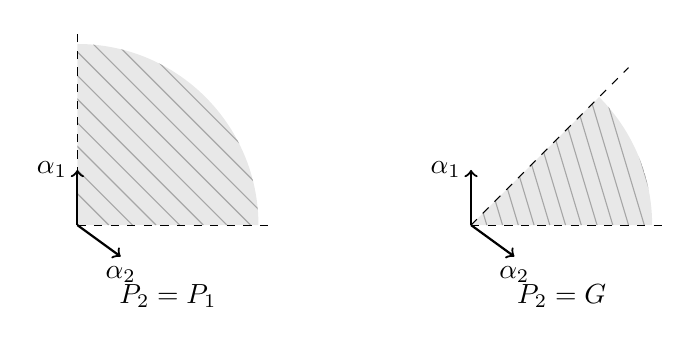
\begin{tikzpicture}[scale=1.0]
 \begin{scope}
 \fill[gray!18] (0,0)--(0,2.3) arc[start angle=90,end angle=0,radius=2.3]--cycle;
 \begin{scope}\clip (0,0)--(0,2.3) arc[start angle=90,end angle=0,radius=2.3]--cycle;
 \foreach \t in {-2,-1.7,...,2.3}{\draw[gray!70] (\t,2.4)--(\t+2.4,0);}\end{scope}
 \draw[dashed] (0,0)--(0,2.5);\draw[dashed](0,0)--(2.5,0);
 \draw[->,thick](0,0)--(0,.7) node[left]{$\alpha_1$};
 \draw[->,thick](0,0)--(.55,-.4) node[below]{$\alpha_2$};
 \node at (1.15,-.9){$P_2=P_1$};
 \end{scope}
 \begin{scope}[xshift=5cm]
 \fill[gray!18](0,0)--(2.3,0) arc[start angle=0,end angle=45,radius=2.3]--cycle;
 \begin{scope}\clip (0,0)--(2.3,0) arc[start angle=0,end angle=45,radius=2.3]--cycle;
 \foreach \t in {0,.2,...,2.5}{\draw[gray!70](\t,0)--(\t-.6,2);}\end{scope}
 \draw[dashed](0,0)--(2,2);\draw[dashed](0,0)--(2.5,0);
 \draw[->,thick](0,0)--(0,.7) node[left]{$\alpha_1$};
 \draw[->,thick](0,0)--(.55,-.4) node[below]{$\alpha_2$};
 \node at (1.15,-.9){$P_2=G$};
 \end{scope}
\end{tikzpicture}
\end{center}
下面的引理将图中反映的关系推广到一般情形。
\begin{originaltheorem}{引理 6（Lemma 6）}
设 $H$ 为 $\mathfrak a_Q$ 中与 $\mathfrak z$ 正交的向量。若 $\sigma_Q^1(H)\ne0$，且
$H=H_*+H^*$，$H_*\in\mathfrak a_Q^1$，$H^*\in\mathfrak a_1$，则对每个 $\alpha\in\Phi_Q^1$，有 $\alpha(H_*)>0$，且
$\|H^*\|<c\|H_*\|$，其中 $c$ 仅依赖于 $G$。换言之，$H^*$ 属于一个紧集，而 $H_*$ 属于 $\mathfrak a_Q^1$ 的正室。\footnote{\textbf{译者注（本次校订）：}这里的紧集依赖于 $H_*$，其半径由 $c\|H_*\|$ 控制；当 $H_*$ 趋于无穷时，不能据此断言 $H^*$ 落在同一个固定紧集中。后面的积分估计须保留这一依赖，先控制该区域体积的多项式增长，再利用 Fourier 变换的快速下降。}
\end{originaltheorem}

将 $k^T(x)$ 写为
\[
 \sum_{Q\subset P_1}\sum_{\delta\in Q(\Q)\backslash G(\Q)}
 F^Q(\delta x,T)\sigma_Q^1(H(\delta x)-T)
 \sum_{P:Q\subset P\subset P_1}(-1)^{\dim(A/Z)}K^P(\delta x,\delta x).
\]
$|k^T(x)|$ 在 $Z(\R)^0G(\Q)\backslash G(A)$ 上的积分，以上述 $Q\subset P_1$ 的和为上界；每一项是在 $Q(\Q)Z(\R)^0\backslash G(A)$ 上 $F^Q(x,T)\sigma_Q^1(H(x)-T)$ 与下式乘积的积分：
\begin{equation}
 \left|\sum_{P:Q\subset P\subset P_1}(-1)^{\dim(A/Z)}
 \int_{N(A)}\sum_{\mu\in M(\Q)}f_\xi(x^{-1}n\mu x)\,dn\right|.\tag{1}
\end{equation}
只需考虑第一个因子非零的 $x$。由上一引理，$H_Q(x)$ 在 $\mathfrak a_Q^1$ 上的投影很大。经 $x^{-1}$ 共轭后，任何不属于 $Q(\Q)$ 的 $\mu\in M(\Q)$ 都会被推向无穷远。因为 $f$ 紧支，可选择充分大的 $T$，使 (1) 中有非零贡献的 $\mu$ 只属于
\[
 Q^P=Q(\Q)\cap M(\Q)=M_Q(\Q)N_Q^P(\Q).
\]
因而 (1) 等于
\[
 \left|\sum_{\mu\in M_Q(\Q)}\sum_{P:Q\subset P\subset P_1}
 (-1)^{\dim(A/Z)}\int_{N(A)}\sum_{\nu\in N_Q^P(\Q)}
 f_\xi(x^{-1}\mu\nu nx)\,dn\right|,
\]
并以
\[
 \sum_{\mu\in M_Q(\Q)}\left|\sum_{P:Q\subset P\subset P_1}
 (-1)^{\dim(A/Z)}\int_{N(A)}\sum_{\nu\in N_Q^P(\Q)}
 f_\xi(x^{-1}\mu\nu nx)\,dn\right|
\]
为上界。

回顾 $N_0$ 的 Lie 代数 $\mathfrak n_0$。以 $\langle\ ,\ \rangle$ 表示 $\mathfrak n_0$ 上的典范双线性型。若 $X\in\mathfrak n_0$，令 $e(X)$ 为把 $X$ 加到单位矩阵所得的 $N_0$ 中的矩阵。那么 $e$ 是从 $\mathfrak n_0$ 到 $N_0$ 的一个 $\Q$ 上簇的同构。\footnote{\textbf{译者注（本次校订）：}对一般约化矩阵群，$X\mapsto I+X$ 未必将 $\mathfrak n_0$ 映入 $N_0$。特征零下可统一使用有限多项式形式的指数映射 $\exp X$，它给出幺幂群与其 Lie 代数之间的簇同构；$I+X$ 适用于一般线性群的标准上三角幺幂群等特殊情形。此外，Poisson 求和所需的非退化配对应另行选定，或直接使用 Lie 代数与其对偶之间的自然配对。}令 $\psi$ 为 $A/\Q$ 上的非平凡特征。对 $\mathfrak n_Q^P$ 应用 Poisson 求和公式，可见 (1) 以上式为界：
\[
 \sum_\mu\left|\sum_P(-1)^{\dim(A/Z)}
 \sum_{\zeta\in\mathfrak n_Q^P(\Q)}\int_{\mathfrak n_Q(A)}
 f_\xi(x^{-1}\mu e(X)x)\psi(\langle X,\zeta\rangle)\,dX\right|.
\]
若 $\mathfrak n_Q^1(\Q)'$ 是 $\mathfrak n_Q^1(\Q)$ 中不属于任何
$\mathfrak n_Q^P(\Q)$（$Q\subset P\subsetneq P_1$）的元素之集，则该表达式等于
\[
 \sum_\mu\left|\sum_{\zeta\in\mathfrak n_Q^1(\Q)'}\int_{\mathfrak n_Q(A)}
 f_\xi(x^{-1}\mu e(X)x)\psi(\langle X,\zeta\rangle)\,dX\right|.
\]
因此，$|k^T(x)|$ 的积分以如下各积分关于 $Q\subset P_1$、$\mu\in M_Q(\Q)$ 的和为上界：对
\[
\begin{split}
 (n^*,n_*,a,m,k)\in{}&N_1(\Q)\backslash N_1(A)
 \times N_Q^1(\Q)\backslash N_Q^1(A)\\
 &\times Z(\R)^0\backslash A_Q(\R)^0
 \times A_Q(\R)^0M_Q(\Q)\backslash M_Q(A)\times K
\end{split}
\]
积分函数
\[
\begin{split}
 &F^Q(m,T)\sigma_Q^1(H(a)-T)e^{-2\langle\rho_Q,H(a)\rangle}\\
 &\quad\cdot\sum_{\zeta\in\mathfrak n_Q^1(\Q)'}
 \left|\int_{\mathfrak n_Q(A)}
 f_\xi(k^{-1}m^{-1}a^{-1}n_*^{-1}(n^*)^{-1}\mu e(X)n^*n_*amk)
 \psi(\langle X,\zeta\rangle)\,dX\right|.
\end{split}
\]
$n^*$ 上的积分消去，$k,m$ 上的积分可限制在紧集上。由上一引理，那些使被积函数非零的 $n_*,a$ 所索引的点集 $\{a^{-1}n_*a\}$ 相对紧。因此，存在
$Z(\R)^0\backslash G(A)$ 中的紧集 $C$，使 $|k^T(x)|$ 的积分以关于
$Q\subset P_1$、$\mu\in M_Q(\Q)$ 的和，以及对 $x\in C$ 的下式积分为上界：
\[
\begin{split}
 &\int_{Z(\R)^0\backslash A_Q(\R)^0}
 e^{-2\langle\rho_Q,H(a)\rangle}\sigma_Q^1(H(a)-T)
 \sum_{\zeta\in\mathfrak n_Q^1(\Q)'}
 \left|\int_{\mathfrak n_Q(A)}f_\xi(x^{-1}\mu a^{-1}e(X)ax)
 \psi(\langle X,\zeta\rangle)\,dX\right|\,da\\
 &=\int_{Z(\R)^0\backslash A_Q(\R)^0}\sigma_Q^1(H(a)-T)
 \sum_\zeta\left|\int_{\mathfrak n_Q(A)}f_\xi(x^{-1}\mu e(X)x)
 \psi(\langle X,\operatorname{Ad}(a)\zeta\rangle)\,dX\right|\,da.
\end{split}
\]
因为 $f$ 紧支，关于 $\mu$ 的和有限。若 $Q=P_1$，则 $\sigma_Q^1=0$，但 $Q=P_1=G$ 时例外，此时它等于 $1$。若 $Q\ne P_1$，则
\[
 Y\longmapsto\int_{\mathfrak n_Q(A)}f_\xi(x^{-1}\mu e(X)x)
 \psi(\langle X,Y\rangle)\,dX,\qquad Y\in\mathfrak n_Q^1(A),
\]
是 $\mathfrak n_Q^1(A)$ 上一个 Schwartz--Bruhat 函数的 Fourier 变换，并关于 $x$ 连续。若
$H(a)=H_*+H^*$，$H_*\in\mathfrak a_Q^1$，$H^*\in\mathfrak a_1/\mathfrak z$，则 $H^*$ 必留在紧集中。由于 $H_*$ 位于远离墙的正室内，$\operatorname{Ad}(a)$ 拉长
$\mathfrak n_Q^1(\Q)'$ 中的任何元素 $\zeta$。事实上，只要 $H_*$ 沿任意方向趋于无穷，$\operatorname{Ad}(a)\zeta$ 也趋于无穷。这里关键是 $\zeta$ 不属于任何
$\mathfrak n_Q^P(\Q)$（$Q\subset P\subsetneq P_1$）。所以 $Q\ne P_1$ 时，相应积分有限，并随 $T$ 增大而指数衰减。因此，唯一剩下的主导项对应于
$Q=P_1=G$，它是紧集 $G(T)$ 上的积分。以上概述了如下定理的证明。

\begin{originaltheorem}{定理 1（Theorem 1）}
可选择 $\varepsilon>0$，使对任意充分远离墙的 $T\in\mathfrak a_0^+$，有
\[
 \int_{Z(\R)^0G(\Q)\backslash G(A)}k^T(x)\,dx
 =\int_{G(T)}K(x,x)\,dx+O(e^{-\varepsilon\|T\|}).
\]
\end{originaltheorem}

自然会想到将 $k^T(x)$ 的积分分解为对应于 $G(\Q)$ 中共轭类的各项之和。不过，$G(\Q)$ 中某种比共轭更弱的等价关系似乎更合适。若 $\mu\in G(\Q)$，以 $\mu_s$ 表示其 Jordan 分解（Jordan decomposition）的半单分量（semisimple component）。若 $\mu_s,\mu_s'$ 在 $G(\Q)$ 中共轭，就称 $\mu,\mu'$ 等价。令 $\mathcal C$ 为这些等价类的集合。若 $\mathfrak o\in\mathcal C$，定义
\[
 K_\mathfrak o^P(x,y)=\sum_{\mu\in M(\Q)\cap\mathfrak o}
 \int_{N(A)}f_\xi(x^{-1}\mu ny)\,dn,
\]
以及
\[
 k_\mathfrak o^T(x)=\sum_P(-1)^{\dim(A/Z)}
 \sum_{\delta\in P(\Q)\backslash G(\Q)}K_\mathfrak o^P(\delta x,\delta x)
 \widehat\tau_P(H(\delta x)-T).
\]
于是 $k^T(x)=\sum_{\mathfrak o\in\mathcal C}k_\mathfrak o^T(x)$。

若 $\mu\in G$，$H$ 为 $G$ 的闭子群，以 $H_\mu$ 表示 $\mu$ 在 $H$ 中的中心化子（centralizer）。
\begin{originaltheorem}{引理 7（Lemma 7）}
固定 $P$。对 $\mu\in M(\Q)$ 和 $\phi\in C_c^\infty(N(A))$，
\[
 \sum_{\zeta\in N_{\mu_s}(\Q)\backslash N(\Q)}
 \sum_{\nu\in N_{\mu_s}(\Q)}
 \phi(\mu^{-1}\zeta^{-1}\mu\nu\zeta)=\sum_{\nu\in N(\Q)}\phi(\nu).
\]
\end{originaltheorem}
引理易证。它蕴含对 $\mathfrak o\in\mathcal C$，有
$P(\Q)\cap\mathfrak o=(M(\Q)\cap\mathfrak o)N(\Q)$。把此事实与定理1的证明结合，得到更强的结论。
\begin{originaltheorem}{定理 $1^*$（Theorem $1^*$）}
存在正常数 $C,\varepsilon$，使
\[
 \sum_{\mathfrak o\in\mathcal C}\int_{Z(\R)^0G(\Q)\backslash G(A)}
 |k_\mathfrak o^T(x)-F^G(x,T)K_\mathfrak o^G(x,x)|\,dx
 \le Ce^{-\varepsilon\|T\|}.
\]
\end{originaltheorem}

为了计算 $k_\mathfrak o^T(x)$ 的积分，需要将它替换为另一个函数。定义
\[
 J_\mathfrak o^P(x,y)=\sum_{\mu\in M(\Q)\cap\mathfrak o}
 \sum_{\zeta\in N_{\mu_s}(\Q)\backslash N(\Q)}
 \int_{N_{\mu_s}(A)}f_\xi(x^{-1}\zeta^{-1}\mu n\zeta y)\,dn.
\]
这是在 $K_\mathfrak o^P(x,y)$ 中，将 $N(A)$ 上的部分积分换为相应的 $\Q$ 有理点求和而得。定义
\[
 j_\mathfrak o^T(x)=\sum_P(-1)^{\dim(A/Z)}
 \sum_{\delta\in P(\Q)\backslash G(\Q)}J_\mathfrak o^P(\delta x,\delta x)
 \widehat\tau_P(H(\delta x)-T).
\]
下面定理的证明与定理 $1^*$ 相似。
\begin{originaltheorem}{定理 2（Theorem 2）}
存在正常数 $C,\varepsilon$，使
\[
 \sum_{\mathfrak o\in\mathcal C}\int_{Z(\R)^0G(\Q)\backslash G(A)}
 |j_\mathfrak o^T(x)-F^G(x,T)K_\mathfrak o^G(x,x)|\,dx
 \le Ce^{-\varepsilon\|T\|}.
\]
\end{originaltheorem}

设 $T_1\in T+\mathfrak a_0^+$。对 $k_\mathfrak o^T(x)$ 与 $k_\mathfrak o^{T_1}(x)$ 的差积分，可归纳证明 $k_\mathfrak o^T(x)$ 的积分是 $T$ 的多项式。$j_\mathfrak o^T(x)$ 的积分同样如此。由于二者之差在 $T\to\infty$ 时趋于零，它们必相等。综上得到：
\begin{originaltheorem}{定理 3（Theorem 3）}
\[
 \int_{Z(\R)^0G(\Q)\backslash G(A)}k^T(x)\,dx
 =\sum_\mathfrak oJ_\mathfrak o^T(f_\xi),
 \qquad J_\mathfrak o^T(f_\xi)=\int_{Z(\R)^0G(\Q)\backslash G(A)}j_\mathfrak o^T(x)\,dx.
\]
\end{originaltheorem}

假设类 $\mathfrak o$ 完全由半单元素构成，于是它是一个真正的共轭类。$\mathfrak o$ 中任意元素的中心化子模去中心后各向异性。该中心的分裂分量在 $G(\Q)$ 中共轭于一个标准抛物子群的分裂分量。因此，可找到 $\mu_\mathfrak o\in\mathfrak o$ 与标准抛物子群 $P_\mathfrak o$，使 $G_{\mu_\mathfrak o}$ 的单位连通分支包含于 $M_\mathfrak o$，且模去 $A_\mathfrak o$ 后各向异性。若 $G_{\mu_\mathfrak o}$ 本身包含于 $M_\mathfrak o$，称类 $\mathfrak o$ 非分歧（unramified）。假设如此，下面将 $J_\mathfrak o^T(f_\xi)$ 表示为 $f_\xi$ 的加权轨道积分（weighted orbital integral）。

给定任意 $P$，设 $\mu\in\mathfrak o\cap M(\Q)$。同样的论证表明，可选择
$s\in\bigcup_{P_1}\Omega(\mathfrak a_\mathfrak o,\mathfrak a_1)$ 与 $\eta\in M(\Q)$，使
$s\mathfrak a_\mathfrak o$ 包含 $\mathfrak a$，且
$\mu=\eta w_s\mu_\mathfrak ow_s^{-1}\eta^{-1}$。令
$\Omega(\mathfrak a_\mathfrak o;P)$ 为上述并集中满足以下条件的 $s$ 的集合：若
$\mathfrak a_1=s\mathfrak a_\mathfrak o$，则 $\mathfrak a_1$ 包含 $\mathfrak a$，并对每个根
$\alpha\in\Phi_{P_1}^P$，$s^{-1}\alpha$ 为正。要求所选 $s$ 属于这个集合后，它就唯一确定。于是 $J_\mathfrak o^P(\delta x,\delta x)$ 等于
\[
\begin{aligned}
 &\sum_{s\in\Omega(\mathfrak a_\mathfrak o;P)}
 \sum_{\eta\in M_{w_s\mu_\mathfrak ow_s^{-1}}(\Q)\backslash M(\Q)}
 \sum_{\zeta\in N(\Q)}
 f_\xi(x^{-1}\delta^{-1}\zeta^{-1}\eta^{-1}w_s\mu_\mathfrak ow_s^{-1}\eta\zeta\delta x)\\
 &=\sum_{s\in\Omega(\mathfrak a_\mathfrak o;P)}
 \sum_{\zeta\in M_{w_s\mu_\mathfrak ow_s^{-1}}(\Q)\backslash P(\Q)}
 f_\xi(x^{-1}\delta^{-1}\zeta^{-1}w_s\mu_\mathfrak ow_s^{-1}\zeta\delta x).
\end{aligned}
\]
因此，$j_\mathfrak o^T(x)$ 等于
\[
 \sum_P(-1)^{\dim(A/Z)}\sum_{s\in\Omega(\mathfrak a_\mathfrak o;P)}
 \sum_{\delta\in M_{w_s\mu_\mathfrak ow_s^{-1}}(\Q)\backslash G(\Q)}
 f_\xi(x^{-1}\delta^{-1}w_s\mu_\mathfrak ow_s^{-1}\delta x)
 \widehat\tau_P(H(\delta x)-T).
\]
由于 $w_s\mu_\mathfrak ow_s^{-1}$ 在 $G$ 中的中心化子包含于 $M$，该式等于
\[
 \sum_{\delta\in G_{\mu_\mathfrak o}(\Q)\backslash G(\Q)}
 f_\xi(x^{-1}\delta^{-1}\mu_\mathfrak o\delta x)
 \sum_P(-1)^{\dim(A/Z)}\sum_{s\in\Omega(\mathfrak a_\mathfrak o;P)}
 \widehat\tau_P(H(w_s\delta x)-T).
\]
于是 $J_\mathfrak o^T(f_\xi)$ 等于
\begin{equation}
 \operatorname{vol}\bigl(A_\mathfrak o(\R)^0G_{\mu_\mathfrak o}(\Q)
 \backslash G_{\mu_\mathfrak o}(A)\bigr)
 \int_{G_{\mu_\mathfrak o}(A)\backslash G(A)}
 f_\xi(x^{-1}\mu_\mathfrak ox)v(x,T)\,dx,\tag{2}
\end{equation}
其中
\[
 v(x,T)=\int_{Z(\R)^0\backslash A_\mathfrak o(\R)^0}
 \left\{\sum_P(-1)^{\dim(A/Z)}\sum_{s\in\Omega(\mathfrak a_\mathfrak o;P)}
 \widehat\tau_P(H(w_sax)-T)\right\}\,da.
\]
括号内的表达式关于 $a$ 紧支。事实上，由 [7，第2、3节] 可知，$v(x,T)$ 等于
\[
 \{s^{-1}T-s^{-1}H(w_sx):s\in\bigcup_{P_1}\Omega(\mathfrak a_\mathfrak o,\mathfrak a_1)\}
\]
在 $\mathfrak a_\mathfrak o/\mathfrak z$ 上投影的凸包（convex hull）的体积。凸包体积会出现在迹公式中，正是 Langlands 曾提出的猜想。

通过研究 $J_\mathfrak o^T(f_\xi)$ 偏离不变分布（invariant distribution）的程度，我希望把一般 $\mathfrak o$ 的 $J_\mathfrak o^T$ 表为上述非分歧类所对应分布的极限，至少模去一个支撑于 $G(A)$ 幺幂集上的不变分布后如此。不过，这还没有完成。

对 $K_E(x,x)$ 的分析采用类似的方法。现在由 $\{\chi\in\mathcal S_E(G)\}$ 代替
$\{\mathfrak o\in\mathcal C\}$。给定 $P$ 和 $\chi\in\mathcal S_E(G)$，定义
\[
\begin{split}
 K_\chi^P(x,y)={}&\sum_{Q\subset P}n^P(A_Q)^{-1}
 \left(\frac1{2\pi i}\right)^{\dim(A_Q/Z)}\\
 &\quad\times\int_{i\mathfrak a_Q^G}\Bigl\{\sum_{\Phi\in\mathcal B_{Q,\chi}}
 E^P(x,I_Q(\Lambda_\xi,f)\Phi,\Lambda)
 \overline{E^P(y,\Phi,\Lambda)}\Bigr\}\,d\Lambda,
\end{split}
\]
其中 $n^P(A_Q)$ 是 $\mathfrak a_Q/\mathfrak a$ 中室的个数。若 $P\ne G$，则
\[
 K^P(x,y)=\sum_{\chi\in\mathcal S_E(G)}K_\chi^P(x,y).
\]
关于 $\chi$ 的和与上述 $\Lambda$ 积分的收敛性由引理2的论证得到。定义
\[
 k_\chi^T(x)=\sum_P(-1)^{\dim(A/Z)}
 \sum_{\delta\in P(\Q)\backslash G(\Q)}K_\chi^P(\delta x,\delta x)
 \widehat\tau_P(H(\delta x)-T).
\]
那么
\[
 K_{\mathrm{cusp}}(x,x)=\sum_{\mathfrak o\in\mathcal C}k_\mathfrak o^T(x)
 -\sum_{\chi\in\mathcal S_E(G)}k_\chi^T(x).
\]
为了计算 $k_\chi^T$ 的积分，仍需先将其替换为新函数 $j_\chi^T$。

为定义新函数，需要引入截断算子（truncation operator）。形式上，它类似于修改 $K(x,x)$ 的方法，但适用于
$Z(\R)^0\cdot G(\Q)\backslash G(A)$ 上任意连续函数 $\phi$。定义该空间上的新函数
\[
 (\Lambda^T\phi)(x)=\sum_{P\supset P_0}(-1)^{\dim(A/Z)}
 \sum_{\delta\in P(\Q)\backslash G(\Q)}\widehat\tau_P(H(\delta x)-T)
 \int_{N(\Q)\backslash N(A)}\phi(n\delta x)\,dn.
\]
$\Lambda^T$ 有一些良好性质：它保持任意尖点形式不变，且为自伴算子（self-adjoint operator）。这些性质可直接验证；进一步还有
$\Lambda^T\circ\Lambda^T=\Lambda^T$。若 $\chi\in\mathcal S_E(G)$，定义
\[
\begin{split}
 J_\chi^T(x,y)=\sum_Pn(A)^{-1}\left(\frac1{2\pi i}\right)^{\dim(A/Z)}
 \int_{i\mathfrak a^G}\left\{\sum_{\Phi\in\mathcal B_{P,\chi}}
 E(x,I_P(\Lambda_\xi,f)\Phi,\Lambda)
 \overline{\Lambda^TE(y,\Phi,\Lambda)}\right\}\,d\Lambda.
\end{split}
\]
把 $\Lambda^T$ 作用于 $K_E(x,y)$ 的第二个变量，得到
$\sum_{\chi\in\mathcal S_E(G)}J_\chi^T(x,y)$。定义 $j_\chi^T(x)=J_\chi^T(x,x)$。

\begin{originaltheorem}{定理 4（Theorem 4）}
函数 $\sum_{\chi\in\mathcal S_E(G)}|j_\chi^T(x)|$ 在
$Z(\R)^0G(\Q)\backslash G(A)$ 上可积。对任意 $\chi$，$j_\chi^T$ 的积分等于
\[
\begin{split}
 &\sum_Pn(A)^{-1}\left(\frac1{2\pi i}\right)^{\dim(A/Z)}
 \int_{i\mathfrak a^G}\sum_{\Phi\in\mathcal B_{P,\chi}}\\
 &\quad\times\int_{Z(\R)^0G(\Q)\backslash G(A)}
 \Lambda^TE(x,I_P(\Lambda_\xi,f)\Phi,\Lambda)
 \overline{\Lambda^TE(x,\Phi,\Lambda)}\,dx\,d\Lambda.
\end{split}
\]
\end{originaltheorem}
定理第一句来自 $\Lambda^T$ 的一个性质：若 $\phi$ 是该商空间上的光滑函数，且其关于
$\mathfrak g(\C)$ 的泛包络代数的任意导数，在某种意义下都缓慢增长，则 $\Lambda^T\phi$ 快速下降（rapidly decreasing）。该性质的证明类似于定理2，但不再使用 Poisson 公式，而改用 [3，引理10]。鉴于 $\Lambda^T\circ\Lambda^T=\Lambda^T$，定理的另一部分归结为交换 $x$ 与 $\Lambda$ 的积分次序。由引理2的证明，本质上可假设被积函数非负，结论随之成立。

\begin{originaltheorem}{定理 5（Theorem 5）}
存在正常数 $C,\varepsilon$，使
\[
 \sum_{\chi\in\mathcal S_E(G)}\int_{Z(\R)^0G(\Q)\backslash G(A)}
 |k_\chi^T(x)-j_\chi^T(x)|\,dx\le Ce^{-\varepsilon\|T\|}.
\]
\end{originaltheorem}
该定理可通过研究在 $x=y$ 处的函数 $k^T(x)-\Lambda^TK(x,y)$ 证明。它本质上是上述被积函数对所有 $\chi$ 的和，不过去掉绝对值。关键是，新函数用 $f$ 表示时具有容易处理的形式，因而更便于研究。

结合定理4、5可见，$\int\sum_{\chi\in\mathcal S_E(G)}|k_\chi^T(x)|\,dx$ 有限；特别地，每个 $k_\chi^T$ 可积。进一步还可以证明 $k_\chi^T$ 与 $j_\chi^T$ 的积分相等。以 $J_\chi^T(f_\xi)$ 表示共同的值，它是 $T$ 的多项式。我们已证明，对适当大的 $T\in\mathfrak a_0^+$，有
\[
 \operatorname{tr}R_{\mathrm{cusp},\xi}(f)
 =\sum_{\mathfrak o\in\mathcal C}J_\mathfrak o^T(f_\xi)
 -\sum_{\chi\in\mathcal S_E(G)}J_\chi^T(f_\xi).
\]
右端是 $T$ 的多项式，左端与 $T$ 无关。令 $J_\mathfrak o(f_\xi)$ 与 $J_\chi(f_\xi)$ 分别为这两个多项式的常数项，得到：
\begin{originaltheorem}{定理 6（Theorem 6）}
对任意 $f\in C_c^\infty(G(A))^K$，
\[
 \operatorname{tr}R_{\mathrm{cusp},\xi}(f)
 =\sum_{\mathfrak o\in\mathcal C}J_\mathfrak o(f_\xi)
 -\sum_{\chi\in\mathcal S_E(G)}J_\chi(f_\xi).
\]
\end{originaltheorem}

设 $\chi=(\mathcal P,\mathcal V,W)$，$P\in\mathcal P$。若 $\Phi\in\mathcal H_{P,\chi}$，则
$\Lambda^TE(x,\Phi,\Lambda)$ 等于 Langlands 在 [2，第9节] 中记作 $E''(x,\Phi,\Lambda)$ 的函数。事实上，截断算子 $\Lambda^T$ 的定义正是受这个函数的启发。若 $\Phi'$ 是 $\mathcal H_{P,\chi}$ 中另一向量，Langlands 证明了优美的公式
\[
\begin{split}
 &\int_{Z(\R)^0G(\Q)\backslash G(A)}
 E''(x,\Phi',\Lambda')\overline{E''(x,\Phi,\Lambda)}\,dx\\
 &=\sum_{P_2}\sum_{t\in\Omega(\mathfrak a,\mathfrak a_2)}
 \sum_{s\in\Omega(\mathfrak a,\mathfrak a_2)}
 \frac{e^{\langle t\Lambda'+s\bar\Lambda,T\rangle}}
 {\prod_{\alpha\in\Phi_2}\langle t\Lambda'+s\bar\Lambda,\alpha\rangle}
 (M(t,\Lambda')\Phi',M(s,\Lambda)\Phi).
\end{split}
\]
见 [2，第9节]。Langlands 原文给出的公式略复杂，但可化为这里的形式。在此公式中，令
$\Lambda'=\Lambda$、$\Phi'=I_P(\Lambda,f)\Phi$，再对 $\mathcal B_{P,\chi}$ 中所有 $\Phi$ 求和，并对 $\Lambda\in i\mathfrak a^G$ 积分。单独对这一相伴类所得的结果还不是 $T$ 的多项式。要得到
$J_\chi^T(f_\xi)$，必须考虑所有 $P$，而不仅是相伴类 $\mathcal P$ 中的 $P$。最有希望的办法似乎是在上式中分别计算关于 $\Lambda$ 和 $\Lambda'$ 的留数。对于 $\operatorname{GL}_3$，结果相对简单。

\origsection{III}{$\operatorname{GL}_3$ 的情形（The case of GL3）}
最后一节给出进一步计算的结果。这些结果可以对一般 $G$ 陈述，但目前只能对
$G=\operatorname{GL}_3$ 证明。目标是用下文定义的不变分布表示
$R_{\mathrm{cusp},\xi}(f)$ 的迹：
\begin{enumerate}
\item[8.] J. Arthur, \emph{On the invariant distributions associated to weighted orbital integrals}, 预印本。
\end{enumerate}
对于 $K$ 双不变函数，迹公式也在下文得到证明：
\begin{enumerate}
\item[9.] A. B. Venkov, \emph{On Selberg's trace formula for $\operatorname{SL}_3(\Z)$}, Soviet Math. Dokl. \textbf{17} (1976), 683--687.
\end{enumerate}

首先，分布 $J_\mathfrak o^T(f_\xi)$ 与 $J_\chi^T(f_\xi)$ 不依赖极小抛物子群的选择，所以不必再固定 $P_0$。若 $A$ 是 $G$ 中任意 $\Q$ 分裂环面，以
$\mathcal P(A)$ 表示分裂分量为 $A$ 的抛物子群集合。它们与 $\mathfrak a$ 中的室一一对应。事实上，若 $P_0$ 是 $\mathcal P(A)$ 中某个元素 $P$ 所含的极小抛物子群，则
\[
 \mathcal P(A)=\bigcup_{A_1}\bigcup_{s\in\Omega(\mathfrak a,\mathfrak a_1)}w_s^{-1}P_1w_s.
\]
若 $P'\in\mathcal P(A)$，且 $P'=w_s^{-1}P_1w_s$，定义
\[
 (M_{P'|P}(\Lambda)\Phi)(x)=(M(s,\Lambda)\Phi)(w_sx),\qquad\Phi\in\mathcal H(P).
\]
那么 $M_{P'|P}(\Lambda)$ 是从 $\mathcal H(P)$ 到 $\mathcal H(P')$ 的映射，与 $P_0$ 无关。事实上，若
$\operatorname{Re}\Lambda\in\rho_P+\mathfrak a_P^+$，则
\begin{equation}
\begin{split}
 (M_{P'|P}(\Lambda)\Phi)(x)
 =\int_{(N(A)\cap N'(A))\backslash N'(A)}
 \Phi(nx)e^{\langle\Lambda+\rho_P,H_P(nx)\rangle}
 e^{-\langle\Lambda+\rho_{P'},H_{P'}(x)\rangle}\,dn.
\end{split}\tag{1}
\end{equation}
这里改用了与 [8] 一致的记号。

若 $\mathcal P(A)$ 非空，称 $A$ 为 $G$ 的特殊子群（special subgroup）。设 $A,A_1$ 为特殊子群，且 $A\supset A_1$。以
$\Omega^{M_1}(\mathfrak a,\mathfrak a)_{\mathrm{reg}}$ 表示
$\Omega(\mathfrak a,\mathfrak a)$ 中在 $\mathfrak a$ 中的不动向量空间恰为 $\mathfrak a_1$ 的元素 $s$ 的集合。设 $P_1\in\mathcal P(A_1)$，
$Q\in\mathcal P^{M_1}(A)$，后者为 $M_1$ 中分裂分量为 $A$ 的抛物子群集合。存在
$\mathcal P(A)$ 中唯一的群 $P_1(Q)$，使 $P_1(Q)\subset P_1$ 且 $P_1(Q)\cap M_1=Q$。

\begin{originaltheorem}{引理 1（Lemma 1）}
设 $A,A_1$ 如上，并且对某些 $P_1\in\mathcal P(A_1)$、$Q\in\mathcal P^{M_1}(A)$，有
$P=P_1(Q)$。若 $\Lambda\in i\mathfrak a_1$，则
\[
 \sum_{P_1\in\mathcal P(A_1)}
 M_{P_1(Q)|P}(\Lambda)^{-1}M_{P_1(Q)|P}(\Lambda+\lambda)
 \left(\prod_{\alpha\in\Phi_{P_1}}\langle\lambda,\alpha\rangle\right)^{-1}
\]
在 $\lambda\to0$ 时，作为 $\mathcal H_P$ 上的算子存在极限。以 $M(P,A_1,\Lambda)$ 表示它。
\end{originaltheorem}
该引理来自 [8]。

固定 $G$ 的一个极大特殊子群 $A_0$。由第二部分末尾引用的 Langlands 内积公式，可证明：
\begin{originaltheorem}{引理 2（Lemma 2）}
对任意 $\chi\in\mathcal S_E(G)$，$J_\chi(f_\xi)$ 等于下式对所有满足
$A_1\subset A\subset A_0$ 的特殊子群 $A_1,A$ 以及
$s\in\Omega^{M_1}(\mathfrak a,\mathfrak a)_{\mathrm{reg}}$ 的和：
\[
 c_s\int_{i\mathfrak a_1^G}\sum_{\Phi\in\mathcal B_{P,\chi}}
 (M(P,A_1,\Lambda_\xi)M(s,0)I_P(\Lambda_\xi,f)\Phi,\Phi)\,d\Lambda.
\]
其中 $c_s$ 是
\[
 \left(\frac1{2\pi i}\right)^{\dim(A_1/Z)}
 n^{M}(A_0)n(A_0)^{-1}
 |\det(1-\operatorname{Ad}(s))_{\mathfrak a/\mathfrak a_1}|^{-1}
\]
与 $\mathfrak a_P^1$ 对 $\Phi_P^1$ 生成的格取商所得体积的乘积；$P$ 可为
$\mathcal P(A_1)$ 中包含 $\mathcal P(A)$ 的某个群的任意元素。
\end{originaltheorem}

回忆分解 $I_P(\Lambda)=\bigoplus_\iota\bigotimes_vI_P(\sigma_v^\iota,\Lambda)$。若
$\Phi_v$ 是 $\mathcal H_P(\sigma_v^\iota)$ 中的光滑向量，且
$\operatorname{Re}\Lambda\in\rho_P+\mathfrak a_P^+$，定义
\[
\begin{split}
 (M_{P'|P}(\sigma_{v,\Lambda}^\iota)\Phi_v)(x)
 =\int_{(N(\Q_v)\cap N'(\Q_v))\backslash N'(\Q_v)}
 \Phi_v(nx)e^{\langle\Lambda+\rho_P,H_P(nx)\rangle}
 e^{-\langle\Lambda+\rho_{P'},H_{P'}(x)\rangle}\,dn,
\end{split}
\]
其中 $x\in G(\Q_v)$。这就是局部群的通常的未归一化交织算子（unnormalized intertwining operator）。于是
\[
 M_{P'|P}(\Lambda)=\bigoplus_\iota\bigotimes_vM_{P'|P}(\sigma_{v,\Lambda}^\iota).
\]

\begin{originaltheorem}{引理 3（Lemma 3）}
若 $\sigma_v$ 是 $M(\Q_v)$ 的不可约酉表示，可定义亚纯函数
$r_{P'|P}(\sigma_{v,\Lambda})$，$P,P'\in\mathcal P(A)$，$\Lambda\in\mathfrak a_\C$，使算子
\[
 R_{P'|P}(\sigma_{v,\Lambda})
 =M_{P'|P}(\sigma_{v,\Lambda})r_{P'|P}(\sigma_{v,\Lambda})^{-1}
\]
可关于 $\Lambda$ 解析延拓，并满足函数方程\footnote{\textbf{译者注（本次校订）：}本引理第一个函数方程右端第二因子中的 $\bar\Lambda$ 应为 $\Lambda$，即 $R_{P^{\prime\prime}|P}(\sigma_{v,\Lambda})=R_{P^{\prime\prime}|P^\prime}(\sigma_{v,\Lambda})R_{P^\prime|P}(\sigma_{v,\Lambda})$。共轭参数出现在随后的伴随关系中，而非交织算子的复合关系中。}
\[
 R_{P''|P}(\sigma_{v,\Lambda})
 =R_{P''|P'}(\sigma_{v,\Lambda})R_{P'|P}(\sigma_{v,\bar\Lambda}),
 \qquad P,P',P''\in\mathcal P(A),
\]
以及
\[
 R_{P'|P}(\sigma_{v,\Lambda})^*=R_{P|P'}(\sigma_{v,-\bar\Lambda}).
\]
此外，若 $\sigma_v$ 属第一类，$\Phi_v$ 为 $K_v$ 不变函数，则
$R_{P'|P}(\sigma_{v,\Lambda})\Phi_v=\Phi_v$。
\end{originaltheorem}

设 $\sigma=\bigotimes\sigma_v$ 为 $M(A)$ 的不可约酉表示。若
$\Phi=\bigotimes\Phi_v$ 是 $\mathcal H_P(\sigma)=\bigotimes_v\mathcal H_P(\sigma_v)$ 中的光滑向量，定义
\[
 R_{P'|P}(\sigma)\Phi=\bigotimes_vR_{P'|P}(\sigma_v)\Phi_v.
\]
对几乎所有 $v$，右端向量是 $K_v$ 的特征函数。定义 $M^1$ 为 $M$ 的定义在 $\Q$ 上的有理特征的共同核。则 $M^1$ 定义在 $\Q$ 上，且
$M(A)=M^1(A)A(A)$。\footnote{\textbf{译者注（本次校订）：}这里的阿代尔点等号一般不成立。例如 $M=\GL_3$、$M^1=\SL_3$、$A$ 为标量环面时，右端元素的行列式必为伊代尔的立方，而左端没有这一限制。代数群上的乘积映射是中心同源，不能直接推出其在阿代尔点上满射。第一部分中用 $M(A)^1$ 与 $A(\R)^0$ 得到的分解则成立；其中 $M(A)^1$ 是所有有理特征的绝对值的共同核，与此处的代数群 $M^1$ 不同。}如第二部分，令 $f\in C_c^\infty(G(A))^K$。

\begin{originaltheorem}{引理 4（Lemma 4）}
存在函数 $\phi_A(f)\in C^\infty(M(A))^{K\cap M(A)}$，使
\[
 (m,a)\longmapsto\phi_A(f,ma),\qquad m\in M^1(A),\ a\in A(A),
\]
关于 $m$ 紧支、关于 $a$ 为 Schwartz 函数，并满足：对 $M(A)$ 任意不可约酉表示
$\sigma=\bigotimes\sigma_v$，
\[
 \operatorname{tr}\sigma(\phi_A(f))
 =\lim_{\lambda\to0}\sum_{P'\in\mathcal P(A)}
 \left(\prod_{\alpha\in\Phi_{P'}}\langle\lambda,\alpha\rangle\right)^{-1}
 \operatorname{tr}\bigl(R_{P'|P}(\sigma)^{-1}R_{P'|P}(\sigma_\lambda)I_P(\sigma,f)\bigr).
\]
右端极限存在，并与所固定的 $P\in\mathcal P(A)$ 无关。
\end{originaltheorem}

设 $\mathfrak o$ 是 $G(\Q)$ 中的等价类。那么 $M(\Q)\cap\mathfrak o$ 是有限个（也可能没有）关于群 $M(\Q)$ 的等价类
$\mathfrak o_1^M\cup\cdots\cup\mathfrak o_n^M$ 的并。若 $F_{\mathfrak o^M}$ 是定义在
$M(\Q)$ 的等价类上的函数，记
\[
 F_\mathfrak o=n^M(A_0)n(A_0)^{-1}\sum_{i=1}^nF_{\mathfrak o_i^M}.
\]
现在为每个 $\mathfrak o\in\mathcal C$ 定义不变分布 $I_\mathfrak o$。定义采用归纳法：假设对每个
$Z\subsetneq A\subset A_0$ 的特殊子群 $A$，都已定义不变分布 $I_{\mathfrak o^M}^M$。定义
\[
 I_\mathfrak o(f_\xi)=J_\mathfrak o(f_\xi)
 -\sum_{A:Z\subsetneq A\subset A_0}I_\mathfrak o^M(\phi_A(f)_\xi).
\]
\begin{originaltheorem}{引理 5（Lemma 5）}
$I_\mathfrak o$ 不变。
\end{originaltheorem}
这本质上是 [8] 的定理5.3。注意，这个引理对归纳定义必不可少，因为 $\phi_A(f)$ 只在模去
$M(A)$ 元素的共轭后才确定。

设 $\sigma=\bigotimes\sigma_v$ 为 $M(A)$ 的酉自守表示（unitary automorphic representation）。那么
\[
 r_{P'|P}(\sigma)=\prod_vr_{P'|P}(\sigma_v),\qquad P,P'\in\mathcal P(A),
\]
本质上是两个 Euler 乘积的商，通过解析延拓定义。若 $\Lambda\in i\mathfrak a$，令
$r_{P'|P}(\Lambda)$ 为 $\mathcal H_P$ 上的算子，它在 $I_P(\sigma^\iota)$ 决定的子空间上按标量
$r_{P'|P}(\sigma_v^\iota)$ 作用。若 $A\supset A_1$，用引理1中的极限定义
$\mathcal H_P$ 上的算子 $r(P,A_1,\Lambda)$，把其中
\[
 M_{P_1(Q)|P}(\Lambda)^{-1}M_{P_1(Q)|P}(\Lambda+\lambda)
\]
换成
\[
 r_{P_1(Q)|P}(\Lambda)^{-1}r_{P_1(Q)|P}(\Lambda+\lambda).
\]
它与 $G(A)$ 的作用对易。最后，对 $\chi\in\mathcal S_E(G)$，用引理2的
$J_\chi(f_\xi)$ 公式定义 $i_\chi(f_\xi)$，把 $M(P,A_1,\Lambda_\xi)$ 换为
$r(P,A_1,\Lambda_\xi)$。于是 $i_\chi$ 是不变分布。

\begin{originaltheorem}{定理 1（Theorem 1）}
对任意 $f\in C_c^\infty(G(A))^K$，
\[
 \operatorname{tr}R_{\mathrm{cusp},\xi}(f)
 =\sum_{\mathfrak o\in\mathcal C}I_\mathfrak o(f_\xi)
 -\sum_{\chi\in\mathcal S_E(G)}i_\chi(f_\xi).
\]
\end{originaltheorem}

\paragraph*{注（Remark）.}
由第二部分的公式 (2)，若 $\mathfrak o$ 完全由半单元素构成，则 $I_\mathfrak o$ 是 [8] 中研究的不变分布之一。此外，由于 $G=\operatorname{GL}_3$，可以证明，对于任意 $\mathfrak o$，
$I_\mathfrak o$ 都是 [8] 中不变分布的若干极限之和。假设 $f=\prod_vf_v$，且在两个素位 $v$，对 $G$ 中所有满足
$Z(\Q_v)\backslash T(\Q_v)$ 非紧的极大环面 $T$，均有
\[
 \int_{T(\Q_v)\backslash G(\Q_v)}f_v(x^{-1}tx)\,dx=0,
 \qquad t\in T(\Q_v)_{\mathrm{reg}}.
\]
由 [8] 的最后一个定理可知，若给定 $\mathfrak o$ 中存在模去 $Z$ 后为 $\Q$ 椭圆的
（$\Q$-elliptic modulo $Z$）元素 $\gamma$，则
\[
 I_\mathfrak o(f_\xi)=\operatorname{vol}\bigl(Z(\R)^0G_\gamma(\Q)\backslash G_\gamma(A)\bigr)
 \int_{G_\gamma(A)\backslash G(A)}f_\xi(x^{-1}\gamma x)\,dx;
\]
若无此 $\gamma$，则 $I_\mathfrak o(f_\xi)=0$。此外，容易看出每个 $i_\chi(f_\xi)=0$。由此，对于上述 $f$，若 $\{\gamma\}$ 是 $G(\Q)$ 中模中心椭圆元素的
$G(\Q)$ 共轭类的一组代表，则
\[
 \operatorname{tr}R_{\mathrm{cusp},\xi}(f)
 =\sum_{\{\gamma\}}\operatorname{vol}\bigl(Z(\R)^0G_\gamma(\Q)\backslash G_\gamma(A)\bigr)
 \int_{G_\gamma(A)\backslash G(A)}f_\xi(x^{-1}\gamma x)\,dx.
\]

\noindent Duke 大学（Duke University）。
